\documentclass[11pt,a4paper]{article}

\usepackage[a4paper, margin=2.4cm]{geometry}
\usepackage{fontspec}
\usepackage[english]{babel}
\babelfont{rm}{Noto Sans}
\usepackage{amsmath,amssymb,amsfonts,mathtools}
\usepackage{booktabs,array,longtable}
\usepackage{graphicx}
% Build with XeLaTeX or LuaLaTeX: fontspec + bidi + Noto Sans; pdflatex will fail.
\usepackage[table]{xcolor}
\usepackage{enumitem}
\usepackage[hidelinks]{hyperref}

\definecolor{accentblue}{RGB}{24, 78, 119}
\definecolor{headerbg}{RGB}{240, 244, 248}
\definecolor{alertbg}{RGB}{253, 246, 236}

\newcommand{\pos}[1]{\left[#1\right]_{+}}
\newcommand{\clip}[1]{\mathrm{clip}\!\left(#1\right)}
\newcommand{\Inat}{\mathbb{I}_{\mathrm{nat}}}
\newcommand{\Inatt}{\mathbb{I}_{\mathrm{nat},t}}
\newcommand{\AAI}{\mathrm{AAI}}

\title{\textbf{A Multi-Tier Agri-Ecological Optimization Framework with Adaptive State-Dependent Orchestration and Nature-Boundary Gatekeeping}}

\author{
  Osama Ahmed Mohamed Gharib Mohamed Alwaly\\
  \small Department of Computer Engineering, Port Said University, Egypt\\
  \small Correspondence: \texttt{osamagharib04@gmail.com}
}

\date{November 23, 2026}

\begin{document}

\maketitle

\begin{abstract}
Conventional precision agriculture frequently optimizes short-term crop output via linear, single-objective formulations while overlooking cumulative soil degradation, seasonal water depletion, and sensor-network energy overhead. This paper presents a multi-tier agri-ecological optimization framework governed by an adaptive, state-dependent orchestration policy across five coupled subsystems: soil quality ($S$), crop performance ($C$), internet-of-things (IoT) monitoring ($M$), hydrological water balance ($W$), and supplier/infrastructure context ($\mathrm{Sup}$). Rather than assuming autonomous reinforcement learning without training guarantees, we formulate three calibrated strictness regimes parameterized by $\tau \in \{0, 1, 2\}$ (\texttt{AI-Low}, \texttt{AI-Med}, and \texttt{AI-Strict}). The framework resolves four mathematical and operational flaws common in weighted sustainability indices: (i) a positive-part clipped multiplicative soil--crop core $\pos{S_{\mathrm{net}}}\pos{C_{\mathrm{net}}}$ that prevents simultaneous degradation from yielding a positive product; (ii) a strictly non-decreasing degradation penalty map $\psi_\tau(x)$ on $[0,1]$ so higher strictness never under-penalizes normalized stress; (iii) disambiguated water storage ($\theta_{\mathrm{root},t}$) and one-sided depletion flux ($D_t^+$); and (iv) an explicit nature-boundary gate $\Inat^{(\tau)}$ paired with a deterministic drought triage fallback policy. Finally, we specify and execute a seed-controlled 52-week benchmark with a six-week late-summer drought (Weeks~24--29) against \emph{two} conventional baselines---fixed-rate and ET-scheduled irrigation---plus the three strictness tiers. Across 20 seeds, ET-scheduled irrigation alone delivers the entire water saving ($8580 \to 5383$\,m$^3$/ha, $-37\%$) and yield gain ($5.76 \to 6.41$\,t/ha) relative to fixed-rate scheduling; adaptive duty cycling then lowers IoT energy from $131.0$ to $16.7$--$17.5$\,kWh/ha ($-87\%$) with no further change in water or yield. The strictness ladder is a genuine trade-off: $\Delta$SOC rises from $-0.18$ to $+1.69$\,g/kg and crop-loss events fall from $8.90$ to $4.40$ crop-weeks, while yield declines to $5.49$\,t/ha at $\tau=2$. Paired $t$-tests support the differences, and all four headline conclusions survive 20 one-at-a-time coefficient perturbations.
\end{abstract}

\noindent\textbf{Keywords:} Agri-ecological optimization; Adaptive state-dependent control; Nature-boundary gatekeeping; IoT duty-cycling; Hydrological water balance; Regenerative agriculture.

%----------------------------------------------------------------------
\section{Introduction}
%----------------------------------------------------------------------
Agricultural production systems operate across heterogeneous pedoclimatic conditions where maximizing yield in isolation can erode long-term ecological capital. Three recurring failure modes motivate a coupled system formulation:
\begin{enumerate}
  \item \textbf{Soil depletion ($S$):} Driven by excessive synthetic inputs, intensive tillage, and organic-matter loss, leading to structural compaction and declining fertility over multi-year horizons.
  \item \textbf{Seasonal water scarcity ($W$):} Exacerbated by heatwaves and climate variability, resulting in root-zone moisture deficits and acute crop water stress when supply falls below evapotranspiration demand.
  \item \textbf{Sensor-network environmental footprint ($M$):} Driven by continuous hardware polling, battery replacements, and device turnover, contributing to operational energy demand and electronic waste.
\end{enumerate}

Passive or purely predictive decision-support tools often fall short in dynamic field environments because they decouple forecasting from physical execution, introduce manual interpretation lag, or rely on open-loop schedules without feedback. Here, we formalize an \emph{adaptive, state-dependent orchestration policy}---a deterministic rule-and-feedback controller that maps real-time telemetry to bounded actuation signals, event-driven sensor duty-cycling, and explicit ecological safety guardrails.

This paper makes four concrete contributions:
\begin{enumerate}
  \item \textbf{Unified Multi-Tier Objective Family ($\tau \in \{0,1,2\}$):} We define a single parameterized objective family spanning \texttt{AI-Low} ($\tau=0$, transitional/compensatory), \texttt{AI-Med} ($\tau=1$, balanced regenerative), and \texttt{AI-Strict} ($\tau=2$, zero-compromise nature-locked). We combine positive-part clipping $\pos{x} = \max(x, 0)$ with a strictly monotone strictness penalty $\psi_2(x) = 1 - (1 - x)^2 \ge x$ on $[0,1]$ so that \texttt{AI-Strict} penalizes degradation at least as strongly as \texttt{AI-Med} across the entire unit interval.
  \item \textbf{State-Dependent IoT Duty-Cycle and Hydrological Coupling:} We bound orchestration scaling factors $\beta_{\AAI}, \phi_{\AAI} \in [1, 5]$ as deterministic functions of observable telemetry and infrastructure readiness, preventing artificial score inflation while linking polling frequency and irrigation allocation to field transients and seasonal evapotranspiration.
  \item \textbf{Hard Ecological Constraints and Deterministic Drought Fallback:} We define the exact gating behaviour of the nature indicator $\Inatt^{(\tau)}$ and specify an operational triage update rule when drought prevents meeting critical root-zone moisture floors.
  \item \textbf{Disambiguated Hydrological Storage and Flux:} We separate weekly depletion flux $D_t$ ($\mathrm{m}^3/\mathrm{week}$) from per-crop root-zone storage $\theta_{\mathrm{root},k,t}$ ($\mathrm{m}^3$), define one-sided depletion $D_t^+=\pos{D_t}$, and give a per-crop storage recursion with field-capacity clipping and explicit deep percolation.
\end{enumerate}

%----------------------------------------------------------------------
\section{Related Work}
%----------------------------------------------------------------------
Prior studies have advanced individual pillars of sustainable agriculture, energy-aware sensing, and safety-constrained water management, yet gaps remain when coupling biophysical soil/crop dynamics, IoT energy management, and non-compensatory ecological boundaries (Table~\ref{tab:lit_comparison}):

\begin{itemize}
  \item \textbf{Regenerative production and social--ecological frameworks:} Karakatsanis et al.~\cite{karakatsanis_2026} formulate REGENA as a structural production function for regenerative farming, consistent with the second law of thermodynamics and the underlying biophysical processes of ecosystem-service generation, and test it on experimental plots in six Mediterranean countries. Buckton et al.~\cite{buckton_2023} articulate a cross-disciplinary conceptual framework for regenerative social--ecological systems. While both inform the theoretical framing of regenerative systems, neither couples ecological boundaries to event-driven IoT duty-cycling.
  \item \textbf{Energy-aware IoT duty-cycling and agricultural sensing:} Gerndt et al.~\cite{gerndt_2025} adapt the duty cycle of solar-powered IoT devices to predicted solar-energy availability---illustrated by a case study that reacts to a forecast sequence of cloudy days---so that continuous operation is maintained. Dhall and Agrawal~\cite{dhall_2018} examine energy-efficient duty-cycling mechanisms tailored to IoT-based precision agriculture networks. These studies focus primarily on node-level energy conservation rather than multi-tier soil--crop--water safety boundaries.
  \item \textbf{Safety-constrained reinforcement learning in irrigation and water management:} Recent work has investigated safety-constrained reinforcement learning for multi-zone irrigation with short-term evapotranspiration forecasting (Fu et al.~\cite{water_2026}), reinforcement learning-based agricultural fertilization and irrigation under N\textsubscript{2}O emissions and uncertain climate variability (Wang et al.~\cite{agrieng_2025}), and a systematic literature review of reinforcement learning applications in water resource management (K{\aa}ge et al.~\cite{frontiers_water_2025}). Fu et al.\ already employ a learned-policy safety layer based on Top-2 gating and total-flow projection, and Chowdhury~\cite{jalrakshak_2026} implements an explicit trust-state fallback with risk-triggered sensing (below); the contribution of this paper is therefore \emph{not} a gate or a fallback in itself, but a deterministic, analytically specified three-tier ($\tau \in \{0,1,2\}$) objective family with a monotone strictness map $\psi_\tau$ and a priority-ordered drought triage rule across multiple crop groups.
  \item \textbf{Safe operating space and ecological boundaries:} te Wierik et al.~\cite{sos_food_2025} allocate nine planetary boundaries to the food system and find that current food systems lie beyond all nine, supplying the biophysical motivation for explicit nature-boundary constraints. Rockstr\"om et al.~\cite{ca_boundaries_2026} argue that conservation agriculture is the scalable route for returning agriculture within those boundaries. These works define \emph{where} the boundary lies but do not encode it as an actuation gate inside a closed-loop controller.
  \item \textbf{Risk-triggered sensing, sensor trust, and duty-cycling:} Chowdhury~\cite{jalrakshak_2026} uses a root-zone water balance as an integrity reference, quarantines a suspect probe through a trust state machine, irrigates from a model twin, and re-admits the probe only after verification, with sampling triggered by risk rather than a fixed schedule. Ruiz-Guirola et al.~\cite{iot_wakeup_2026} optimise duty cycling and selective wake-up for energy-harvesting IoT networks, and Falamba et al.~\cite{solar_iot_2026} validate a solar-powered IoT drip-irrigation system over a full cultivation cycle. These systems demonstrate integrity checking, event-driven sampling, and field validation, but they do not define an analytically specified tiered objective with a monotone strictness penalty and priority-ordered drought triage across multiple crop groups.
\end{itemize}

\noindent\emph{Scope note:} All twelve bibliography entries cited in this manuscript were verified against DOI records and abstracts (OpenAlex and Crossref) on 23~November~2026.

\begin{table}[t]
  \centering
  \small
  \caption{Qualitative scope comparison across verified literature and the proposed framework.}
  \label{tab:lit_comparison}
  \begin{tabular}{@{}p{3.4cm}p{3.6cm}p{3.6cm}p{3.6cm}@{}}
    \toprule
    \textbf{Reference} & \textbf{Primary Focus} & \textbf{Soil / Water / Sensing Scope} & \textbf{Safety Gate \& Fallback} \\
    \midrule
    Karakatsanis et al.~\cite{karakatsanis_2026} & Structural production function consistent with the 2nd law of thermodynamics (REGENA) & Biophysical and economic modelling of regenerative plots; no IoT polling control & Endogenous regenerative conditions; no automated actuation gate \\
    Buckton et al.~\cite{buckton_2023} & Regenerative social--ecological conceptual framework & Cross-disciplinary socio-ecological principles & Conceptual framing; no closed-loop controller \\
    Gerndt et al.~\cite{gerndt_2025} & Solar-powered IoT duty-cycle management & Node battery state and solar forecast; general IoT & Battery/energy-aware scheduling thresholds \\
    Dhall \& Agrawal~\cite{dhall_2018} & Energy-efficient duty cycling in precision ag IoT & Wireless sensor network energy conservation & Periodic/threshold sleep scheduling \\
    Fu et al.~\cite{water_2026} and Wang et al.~\cite{agrieng_2025} & Safety-constrained RL with ET forecasting; RL under N\textsubscript{2}O uncertainty & Multi-zone irrigation and fertilization policy optimization & Learned/constrained policies without tiered $\Inat$ triage \\
    K{\aa}ge et al.~\cite{frontiers_water_2025} & Systematic review of RL in water management & Overview of RL applications in water resources & No tiered gate or drought triage rule \\
    te Wierik et al.~\cite{sos_food_2025} and Rockstr\"om et al.~\cite{ca_boundaries_2026} & Food-system safe operating space; return within planetary boundaries & Biophysical boundary budgets; no actuation layer & Boundaries defined globally, not as a per-field gate \\
    Chowdhury~\cite{jalrakshak_2026} & Water-balance integrity and risk-triggered sensing (JalRakshak) & Root-zone depletion twin; probe quarantine and re-admission & Trust-state fallback; no tiered objective or multi-crop triage \\
    Ruiz-Guirola et al.~\cite{iot_wakeup_2026} and Falamba et al.~\cite{solar_iot_2026} & Energy-harvesting duty cycling; validated solar IoT irrigation & Node energy scheduling and field sensor validation & No ecological gate or drought triage rule \\
    \textbf{This work} & Multi-tier ($\tau \in \{0,1,2\}$) agri-ecological optimization & Coupled $S, C, M, W, \mathrm{Sup}$ with bounded state control & Explicit $\Inat^{(\tau)}$ gate, hard bounds, and deterministic drought triage \\
    \bottomrule
  \end{tabular}
\end{table}

%----------------------------------------------------------------------
\section{Methodology: Agro-Ecological Efficiency Framework}
%----------------------------------------------------------------------

\subsection{System Variables and Disambiguated Notation}
To prevent unit confusion between hydrological fluxes and soil-water storage, we strictly separate weekly depletion flux ($D_t$, in $\mathrm{m}^3/\text{week}$) from per-crop root-zone water storage ($\theta_{\mathrm{root},k,t}$, in $\mathrm{m}^3$). All state sub-indices are normalized to $[0, 1]$ prior to aggregation:

\begin{itemize}
  \item \textbf{Soil quality ($S \in [0,1]$):} Positive indicators comprise organic matter ($S_{\mathrm{org}}$), microbial activity ($S_{\mathrm{mic}}$), porosity ($S_{\mathrm{por}}$), and available nutrients ($S_{\mathrm{nut}}$), contrasted against normalized soil degradation/compaction ($S_{\mathrm{deg}} \in [0,1]$).
  \item \textbf{Crop performance ($C \in [0,1]$):} Across $K$ crop groups, positive indicators comprise nutritional/yield index ($C_{\mathrm{nut},k}$), functional biodiversity ($C_{\mathrm{bio},k}$), and varietal diversity ($C_{\mathrm{div},k}$), contrasted against normalized external abiotic stress ($C_{\mathrm{ext},k} \in [0,1]$).
  \item \textbf{IoT monitoring ($M \in [0,1]$):} Comprises normalized active electrical draw ($M_{\mathrm{elec}}$), active duty-cycle fraction ($M_{\mathrm{duty}}$), and hardware amortization overhead ($M_{\mathrm{hw}}$).
  \item \textbf{Hydrological water balance ($W$):} At week $t \in \{1,\dots,T\}$, field-wide weekly net water depletion flux is defined as
  \begin{equation}
    D_t = \sum_{k=1}^{K} W_{\mathrm{ext},k,t} + W_{\mathrm{loss},t} - W_{\mathrm{rain},t} \quad [\mathrm{m}^3/\text{week}],
  \end{equation}
  where $W_{\mathrm{ext},k,t}$ is irrigation extraction allocated to crop group $k$ (bounded by total available supply $\sum_{k=1}^K W_{\mathrm{ext},k,t} \le W_{\mathrm{avail},t}$), $W_{\mathrm{loss},t}$ is conveyance/evaporative loss, and $W_{\mathrm{rain},t}$ is effective precipitation. The field has total area $A = 1\,\mathrm{ha}$ partitioned into $K$ equal plots $A_k = A/K$; field-wide rain is apportioned as $W_{\mathrm{rain},k,t} = \alpha_k W_{\mathrm{rain},t}$ with $\alpha_k = 1/K$ and $\sum_k \alpha_k = 1$. Only positive depletion $D_t^+ = \pos{D_t}$ is penalized, normalized by a regional seasonal reference cap $D_{\max} > 0$ so $\tilde{D}_t^+ = \min(D_t^+ / D_{\max}, 1) \in [0,1]$. For each crop group $k \in \{1,\dots,K\}$, root-zone water storage evolves via
  \begin{equation}
    \theta_{\mathrm{root},k,t+1} = \mathrm{clip}\!\left(\theta_{\mathrm{root},k,t} + W_{\mathrm{rain},k,t} + \eta_{\mathrm{irr}} W_{\mathrm{ext},k,t} - \mathrm{ET}_{c,k,t} - W_{\mathrm{perc},k,t},\; 0,\; \theta_{\mathrm{fc},k}\right),
  \end{equation}
  where $\eta_{\mathrm{irr}} \in (0,1]$ is field application efficiency, $\mathrm{ET}_{c,k,t} = 10\,K_{c,k,t}\,\mathrm{ET}_{0,t}\,A_k$ is crop evapotranspiration in $\mathrm{m}^3/\mathrm{week}$, computed from reference evapotranspiration $\mathrm{ET}_{0,t}$ (mm/week), crop coefficient $K_{c,k,t}$, and plot area $A_k$ (ha); the factor $10$ converts one mm over one hectare to $10\,\mathrm{m}^3$, $W_{\mathrm{perc},k,t} = \max(0, \theta_{\mathrm{root},k,t} + W_{\mathrm{rain},k,t} + \eta_{\mathrm{irr}} W_{\mathrm{ext},k,t} - \mathrm{ET}_{c,k,t} - \theta_{\mathrm{fc},k})$ is deep percolation above field capacity $\theta_{\mathrm{fc},k}$, and $\bar{\theta}_{\mathrm{root},t} = \frac{1}{K}\sum_{k=1}^K \theta_{\mathrm{root},k,t}$ denotes mean root-zone storage.
  \item \textbf{Supplier and infrastructure context ($\mathrm{Sup}$):} Captures technology readiness ($\mathrm{Sup}_{\mathrm{tech}} \in [0,1]$), conveyance/distribution efficiency ($\mathrm{Sup}_{\mathrm{dist}} \in [0,1]$), and regulatory compliance burden ($\mathrm{Sup}_{\mathrm{reg}} \in [0,1]$, where higher values indicate stricter compliance overhead).
\end{itemize}

\subsection{State Evolution and Disturbance Model}
The benchmark advances the ecological state each week under the following explicit rules; $\clip{\cdot}$ denotes clipping to the stated domain:
\begin{align}
  S_{\mathrm{org},t+1} &= \clip{S_{\mathrm{org},t} + 0.0018\left(1-C_{\mathrm{chem}}/120\right) - 0.0010\,D_t^+/D_{\max}},\\
  S_{\mathrm{deg},t+1} &= \clip{S_{\mathrm{deg},t} + 0.0015\,C_{\mathrm{chem}}/120 + 0.0008\,D_t^+/D_{\max} - 0.0012\,S_{\mathrm{org},t}},\\
  S_{i,t} &= \left(S_{\mathrm{org},t},\,0.8S_{\mathrm{org},t}+0.1,\,0.7S_{\mathrm{org},t}+0.2,\,0.6S_{\mathrm{org},t}+0.3\right),\\
  C_{\mathrm{ext},k,t} &= \clip{0.2+0.6\,\pos{\theta_{\mathrm{crit},k}-\theta_{\mathrm{root},k,t}}/\theta_{\mathrm{crit},k} + \mathbb{1}_{t\in\mathcal{D}}\,0.35},\\
  C_{j,k,t} &= \clip{C^{\mathrm{base}}_{j,k}\left(0.6+0.4\,\theta_{\mathrm{root},k,t}/\theta_{\mathrm{fc},k}\right)}.
\end{align}
Here $\mathcal{D}=\{24,\dots,29\}$ is the drought window and $C^{\mathrm{base}}$ is the $3\times3$ matrix of baseline crop-indicator values given in Table~\ref{tab:full_params}. The drought disturbance is a \emph{level shift}: $+0.35$ on $C_{\mathrm{ext},k,t}$ and $+0.38$ on the effective soil degradation $S_{\mathrm{deg},t}^{\mathrm{eff}}=S_{\mathrm{deg},t}+\mathbb{1}_{t\in\mathcal{D}}0.38$ during the six weeks only, reverting afterwards. This interpretation avoids an unbounded six-fold accumulation of the shock. Actual evapotranspiration is $\mathrm{ETa}_{k,t}=\min\!\left(\mathrm{ET}_{c,k,t},\,\pos{\theta_{\mathrm{root},k,t}+W_{\mathrm{rain},k,t}+\eta_{\mathrm{irr}}W_{\mathrm{ext},k,t}}\right)$, giving the yield response in Eq.~\eqref{eq:yield}:
\begin{equation}
  Y_k = Y_k^{\max}\,\frac{\sum_t \mathrm{ETa}_{k,t}}{\sum_t \mathrm{ET}_{c,k,t}}\left(0.85+0.15\,\frac{C_{\mathrm{chem}}}{120}\right),
  \label{eq:yield}
\end{equation}
and cumulative IoT energy $E=\sum_t M_{\mathrm{duty},t}\,P_{\mathrm{node}}\,N_{\mathrm{nodes}}\,h/1000$ with $P_{\mathrm{node}}=0.5$\,W, $N_{\mathrm{nodes}}=30$ and $h=168$\,h/week. All five policies are driven by the same rainfall and thermal draws for a given seed.

\subsection{Bounded State-Dependent Orchestration Logic}
Orchestration scaling factors $\beta_{\AAI,t}$ and $\phi_{\AAI}$ are deterministic functions bounded within $[1.0, 5.0]$, preventing unconstrained score manipulation while aligning penalty relaxation with telemetry demand:
\begin{align}
  \beta_{\AAI,t} &= 1.0 + 4.0\,\Big(1 - \exp\!\left(-\rho_\beta \left(g_{\theta,t} + g_{T,t}\right)\right)\Big) \in [1.0, 5.0], \label{eq:beta_rule} \\
  \phi_{\AAI} &= 1.0 + 4.0\,\mathrm{Sup}_{\mathrm{dist}} \in [1.0, 5.0], \label{eq:phi_rule}
\end{align}
where $g_{\theta,t} = |\Delta\bar\theta_{\mathrm{root},t}|/\bar\theta_{\mathrm{fc}}$ and $g_{T,t} = |\Delta T_{\mathrm{soil},t}|/(10\,^{\circ}\mathrm{C})$ are dimensionless week-over-week gradients, with $\bar\theta_{\mathrm{fc}}=K^{-1}\sum_k\theta_{\mathrm{fc},k}=263.3\,\mathrm{m}^3$ (Table~\ref{tab:full_params}). The duty cycle is
\begin{equation}
  M_{\mathrm{duty},t} = \begin{cases}
    M_{\min}, & \text{drought triage},\\
    \clip{M_{\min}+(M_{\max}-M_{\min})(\beta_{\AAI,t}-1)/4,\;M_{\min},\;M_{\max}}, & \text{otherwise}.
  \end{cases}
  \label{eq:duty_rule}
\end{equation}
 where $\rho_\beta = 3.0$ is a sensitivity constant and $M_{\max}=0.40$ is the polling ceiling. Under steady field conditions ($g_{\theta,t}+g_{T,t}\to0$), $\beta_{\AAI,t}\to1.0$ and $M_{\mathrm{duty},t}\to M_{\min}=0.05$; during rapid transients, $\beta_{\AAI,t}\to5.0$ and $M_{\mathrm{duty},t}\to M_{\max}=0.40$, so polling increases exactly when moisture or thermal gradients are largest. With $M_{\mathrm{elec}}=M_{\mathrm{duty}}=M_{\mathrm{duty},t}$ and $M_{\mathrm{hw}}=0.25$, the normalised sensing penalty $c_M\sum_i\theta_i M_i/\beta_{\AAI,t}$ in Eq.~\eqref{eq:unified_objective} falls from $0.117\,c_M$ at steady state to $0.070\,c_M$ at maximum demand: the denominator relaxes faster than duty rises, so the controller is not penalised for the extra sensing that transients require. Similarly, seasonal water weighting $\omega_t$ follows a sinusoidal evaporative-demand curve:
\begin{equation}
  \omega_t = 1.0 + A_\omega \sin\!\left(\frac{2\pi (t - t_0)}{52}\right), \quad t \in \{1,\dots,52\},
  \label{eq:omega_fao}
\end{equation}
with amplitude $A_\omega = 0.45$ and phase offset $t_0 = 13$ so peak weighting aligns with midsummer radiation and evaporative demand (Weeks~24--29).

\begin{figure}[t]
  \centering
  \includegraphics[width=\linewidth]{figures/fig1\_closed\_loop\_architecture.png}
  \caption{Closed-loop orchestration architecture. Field telemetry ($S,C,M,W,\mathrm{Sup}$) is normalised and mapped by the tier-dependent objective in Eq.~\eqref{eq:unified_objective}; the nature gate $\Inatt^{(\tau)}$ and hard bounds produce actuation signals, with drought triage engaged during Weeks~24--29. Generated by \texttt{generate\_figures.py}; no empirical data are shown.}
  \label{fig:architecture}
\end{figure}

\subsection{Monotone Strictness Penalty and Unified Objective ($\tau \in \{0, 1, 2\}$)}
A critical mathematical pitfall in normalized indices on $[0,1]$ is using $x^p$ with $p > 1$ as a "stricter" penalty: for any $x \in (0,1)$, $x^2 < x$, which would inadvertently \emph{reduce} penalties in the strictest tier. To guarantee monotone strictness across $\tau \in \{0, 1, 2\}$, we define the bounded penalty map $\psi_\tau : [0,1] \to [0,1]$ as:
\begin{equation}
  \psi_\tau(x) = \begin{cases}
    x, & \tau \in \{0, 1\}, \\
    1 - (1 - x)^2 = 2x - x^2, & \tau = 2.
  \end{cases}
  \label{eq:psi_penalty}
\end{equation}
Because $\psi_2(x) - \psi_1(x) = x(1 - x) \ge 0$ for all $x \in [0,1]$ (with strict inequality on $(0,1)$) and $\psi_2'(x) = 2(1-x) \ge 0$, $\psi_2(x)$ is concave, strictly increasing on $[0,1)$, and strictly dominates $\psi_1(x)$ for every non-trivial degradation or depletion level.

\begin{figure}[t]
  \centering
  \includegraphics[width=\linewidth]{figures/fig2\_tier\_progression.png}
  \caption{Strictness-tier progression. Top: the three tier configurations ($m_{\mathrm{mult}}$, $\psi_\tau$, weights and gate). Bottom left and centre: additive versus multiplicative reward cores under positive-part clipping. Bottom right: the monotone penalty maps $\psi_0=\psi_1=x$ and $\psi_2=1-(1-x)^2$, with the shaded gap $x(1-x)\ge 0$ and $\psi_2'(x)=2(1-x)\ge 0$. Generated by \texttt{generate\_figures.py}; no empirical data are shown.}
  \label{fig:tiers}
\end{figure}

Using $\psi_\tau(\cdot)$, we define the net soil index $S_{\mathrm{net},t}^{(\tau)}$ and net crop index $C_{\mathrm{net},t}^{(\tau)}$ across $K$ crop groups at each week $t$ (the drought forcing in Section~5 makes degradation and stress time-varying):
\begin{align}
  S_{\mathrm{net},t}^{(\tau)} &= \sum_{i=1}^{4} \delta_i S_{i,t} - \eta\,\psi_\tau\!\left(S_{\mathrm{deg},t}\right), \\
  C_{\mathrm{net},t}^{(\tau)} &= \frac{1}{K}\sum_{k=1}^{K}\left(\sum_{j=1}^{3} \gamma_j C_{j,k,t} - \lambda\,\psi_\tau\!\left(C_{\mathrm{ext},k,t}\right)\right).
\end{align}
Let $\kappa_t = \frac{1}{3}\left[\mathrm{Sup}_{\mathrm{tech}} + (1 - \mathrm{Sup}_{\mathrm{dist}}) + \mathrm{Sup}_{\mathrm{reg}}\right] \in [0,1]$ denote the normalized supplier/infrastructure cost factor. The unified multi-tier objective $\mathcal{J}_{\tau}$ is:
\begin{align}
  \mathcal{J}_{\tau} &= \frac{1}{T}\sum_{t=1}^{T}\Bigg\{ \Inatt^{(\tau)} \Big[ w_S(\tau)\,\pos{S_{\mathrm{net},t}^{(\tau)}} + w_C(\tau)\,\pos{C_{\mathrm{net},t}^{(\tau)}} + m_{\mathrm{mult}}(\tau)\,\pos{S_{\mathrm{net},t}^{(\tau)}}\,\pos{C_{\mathrm{net},t}^{(\tau)}} \Big] \nonumber\\
  &\quad - c_M(\tau)\,\frac{\sum_{i=1}^{3}\theta_i M_{i,t}}{\beta_{\AAI,t}} - c_W(\tau)\, \frac{\omega_t\,\psi_\tau\!\left(\tilde{D}_t^+\right)\kappa_t}{\phi_{\AAI}} \Bigg\}.
  \label{eq:unified_objective}
\end{align}
Notice that $\Inatt^{(\tau)}$ is evaluated at every week $t$ inside the time average: it gates only the ecological reward core, while the sensing and water penalties remain active in the same summand even during a breach, so excessive water or energy draw during a crisis is never masked. Furthermore, positive-part clipping $\pos{\cdot}$ guarantees that if either $S_{\mathrm{net},t}^{(\tau)} \le 0$ or $C_{\mathrm{net},t}^{(\tau)} \le 0$, the multiplicative term $\pos{S_{\mathrm{net},t}^{(2)}}\pos{C_{\mathrm{net},t}^{(2)}}$ evaluates to $0$ rather than yielding a false positive product from two negative factors.

\subsection{Hard Ecological Constraints and Drought Triage Fallback}
Every feasible policy must satisfy four operational rules:
\begin{enumerate}
  \item \textbf{Tier-scoped chemical input cap:} Synthetic chemical intensity $C_{\mathrm{chem}}$ ($\mathrm{kg/ha}$) satisfies $C_{\mathrm{chem}} \le C_{\mathrm{chem}}^{\max}(\tau)$, where $C_{\mathrm{chem}}^{\max}(0) = 120\,\mathrm{kg/ha}$ (transitional), $C_{\mathrm{chem}}^{\max}(1) = 45\,\mathrm{kg/ha}$ (reduced), and $C_{\mathrm{chem}}^{\max}(2) = 0\,\mathrm{kg/ha}$ (strict organic/regenerative).
  \item \textbf{Bounded sensor duty cycle:} $M_{\min}=0.05 \le M_{\mathrm{duty},t} \le M_{\max}=0.40$ at all weeks $t$: the lower bound preserves baseline observability, the upper bound prevents duty-cycling from becoming a second uncontrolled resource.
  \item \textbf{Normal-operation root-zone moisture floor:} $\theta_{\mathrm{root},k,t} \ge \theta_{\mathrm{crit},k}$ for each crop group $k \in \{1,\dots,K\}$ under normal supply. This is a control target rather than an inviolable physical bound: the drought fallback in rule~4 is a documented exception that intentionally drives one or more crops below $\theta_{\mathrm{crit},k}$, with the resulting violation registered by $\Inatt^{(2)}=0$ rather than being masked.
  \item \textbf{Nature gate $\Inatt^{(\tau)}$ and deterministic drought fallback:} For $\tau \in \{0,1\}$, $\Inatt^{(\tau)} = 1$ at all weeks. For $\tau = 2$ (\texttt{AI-Strict}), Eq.~\eqref{eq:inat_gate} applies:
  \begin{equation}
    \Inatt^{(2)} = \begin{cases}
      0, & \text{if } S_{\mathrm{deg},t} > S_{\mathrm{deg}}^{\mathrm{emerg}} \;\lor\; \min_{k}\left(\theta_{\mathrm{root},k,t} - \theta_{\mathrm{crit},k}\right) < 0, \\
      1, & \text{otherwise},
    \end{cases}
    \label{eq:inat_gate}
  \end{equation}
  where $S_{\mathrm{deg}}^{\mathrm{emerg}} = 0.65$. \textbf{Deterministic fallback update rule:} Whenever drought supply limits prevent satisfying $\theta_{\mathrm{root},k,t} \ge \theta_{\mathrm{crit},k}$ across all plots simultaneously, the controller enters \emph{deficit-rationed triage}: (a) available irrigation water $W_{\mathrm{avail},t}$ is allocated strictly in descending order of crop survival priority (legume cover/perennial rootstock first, followed by winter wheat, then grain maize) capped at survival maintenance $\theta_{\mathrm{surv},k} = 0.85\,\theta_{\mathrm{crit},k}$; (b) sensor duty cycles on non-critical plots clamp to $M_{\min} = 0.05$ to conserve battery energy; (c) $\Inatt^{(2)}$ sets to $0$ (zeroing the ecological reward term while keeping depletion penalties active in Eq.~\eqref{eq:unified_objective}); and (d) normal closed-loop operation resumes automatically at week $t'$ once $\theta_{\mathrm{root},k,t'} \ge \theta_{\mathrm{crit},k}$ and $S_{\mathrm{deg},t'} \le S_{\mathrm{deg}}^{\mathrm{emerg}}$ hold for two consecutive weeks. Thus the triage rule deliberately violates the rule-3 target under scarcity; the gate is the mechanism that registers that controlled violation rather than concealing it.
\end{enumerate}

\begin{table}[t]
  \centering
  \small
  \caption{Complete parameter specification, units, and tier calibration values for reproducible simulation.}
  \label{tab:full_params}
  \resizebox{\linewidth}{!}{%
  \begin{tabular}{@{}llll@{}}
    \toprule
    \textbf{Symbol} & \textbf{Description} & \textbf{Units / Domain} & \textbf{Calibrated Value / Rule} \\
    \midrule
    $\tau$ & Strictness tier index & $\{0, 1, 2\}$ & $0$: \texttt{AI-Low}, $1$: \texttt{AI-Med}, $2$: \texttt{AI-Strict} \\
    $w_S(\tau), w_C(\tau)$ & Linear soil and crop weights & Dimensionless & $(1.0, 1.0)$ for $\tau \in \{0,1\}$; $(0.5, 0.5)$ for $\tau=2$ \\
    $m_{\mathrm{mult}}(\tau)$ & Multiplicative coupling weight & Dimensionless & $0.0$ for $\tau \in \{0,1\}$; $1.5$ for $\tau=2$ \\
    $c_M(\tau), c_W(\tau)$ & Sensing and water penalty weights & Dimensionless & $(0.25, 0.30)_{\tau=0}$; $(0.50, 0.60)_{\tau=1}$; $(0.80, 1.00)_{\tau=2}$ \\
    $\delta_i, \eta$ & Soil sub-weights and degradation weight & Dimensionless & $\delta_i = 0.25\;(i=1\dots 4)$, $\eta = 1.0$ \\
    $\gamma_j, \lambda$ & Crop sub-weights and stress weight & Dimensionless & $\gamma_j = 1/3\;(j=1\dots 3)$, $\lambda = 1.0$ \\
    $\theta_i$ & Monitoring sub-weights & Dimensionless & $\theta_i = 1/3\;(i=1\dots 3)$ \\
    $\beta_{\AAI,t}, \phi_{\AAI}$ & Orchestration scaling factors & $[1.0, 5.0]$ & Eq.~\eqref{eq:beta_rule} ($\rho_\beta = 3.0$) and Eq.~\eqref{eq:phi_rule} \\
    $g_{\theta,t}, g_{T,t}$ & Normalized weekly gradients & dimensionless & $|\Delta\bar\theta_{\rm root,t}|/263.3\,\mathrm{m}^3$; $|\Delta T_{\rm soil,t}|/10\,^{\circ}\mathrm{C}$ \\
    $\omega_t$ & Seasonal evaporative weight & $[0.55, 1.45]$ & Eq.~\eqref{eq:omega_fao} ($A_\omega = 0.45$, $t_0 = 13$) \\
    $\eta_{\mathrm{irr}}, W_{\mathrm{avail},t}$ & Application efficiency and supply cap & $(0,1]$, $\mathrm{m}^3/\text{wk}$ & $\eta_{\mathrm{irr}} = 0.85$; $W_{\mathrm{avail},t} = 600$ ($240$ in drought) \\
    $A, A_k, \alpha_k$ & Field area, plot area, rain apportionment & $\mathrm{ha}$, $\mathrm{ha}$, dimensionless & $A=1$; $A_k=A/K=1/3$; $\alpha_k=1/3$ \\
    $W_{\mathrm{loss},t}$ & Conveyance loss & $\mathrm{m}^3/\text{week}$ & $0.05\sum_k W_{\mathrm{ext},k,t}$ \\
    $\mathrm{ET}_{0,t}$ & Reference evapotranspiration & $\mathrm{mm}/\text{week}$ & $28.5 + 13.5\sin(2\pi(t-13)/52) \in [15,42]$ \\
    $K_{c,k,t}$ & Crop coefficient (wheat, maize, legume) & dimensionless & $0.4+0.7e^{-((t-12)/8)^2}$, $0.4+0.8e^{-((t-26)/9)^2}$, $0.35+0.55e^{-((t-35)/10)^2}$ \\
    $W_{\mathrm{rain},t}$ & Effective rainfall draw & $\mathrm{m}^3/\text{week}$ & $\mathrm{Gamma}(2,\,[120+60\cos(2\pi(t-5)/52)]/2)$, $\times\,0.30$ in drought \\
    $T_{\mathrm{soil},t}$ & Topsoil temperature & $^\circ\mathrm{C}$ & $18 + 10e^{-0.002t}\sin(2\pi(t-13)/52) + \mathcal{N}(0,0.5)$ \\
    $\mathrm{Sup}_{\mathrm{tech}}, \mathrm{Sup}_{\mathrm{dist}}, \mathrm{Sup}_{\mathrm{reg}}$ & Infrastructure context & $[0,1]$ & $0.80$, $0.90$, $0.40$ \\
    $M_{\mathrm{elec},t}, M_{\mathrm{duty},t}, M_{\mathrm{hw}}$ & Normalised monitoring draw & $[0,1]$ & $M_{\mathrm{elec},t}=M_{\mathrm{duty},t}$; $M_{\mathrm{hw}}=0.25$; duty from Eq.~\eqref{eq:duty_rule} \\
    $Y^{\max}_k$ & Potential yield (wheat, maize, legume) & $\mathrm{t}/\mathrm{ha}$ & $7$, $10$, $3$ \\
    $C^{\mathrm{base}}_{j,k}$ & Baseline crop-indicator matrix (rows $j$) & dimensionless & $\left[\begin{smallmatrix}0.75&0.70&0.65\\0.80&0.60&0.55\\0.65&0.85&0.90\end{smallmatrix}\right]$ \\
    $\theta_{\mathrm{fc},k}, \theta_{\mathrm{root},k,0}$ & Field capacity and initial storage & $\mathrm{m}^3$ & Wheat: $260, 210$; Maize: $310, 250$; Legume: $220, 180$ \\
    $\theta_{\mathrm{crit},k}$ & Critical root-zone water floor ($K=3$) & $\mathrm{m}^3$ & Wheat: $180$; Maize: $220$; Legume: $150$ \\
    $\mathrm{ET}_{c,k,t}, T_{\mathrm{soil},t}$ & Crop ET and topsoil temperature & $\mathrm{m}^3/\text{wk}$, $^{\circ}\mathrm{C}$ & Seasonal FAO curve ($\mathrm{ET}_0 \in [15,42]\,\mathrm{mm/wk}$, $T_{\mathrm{soil}} \in [8,28]^{\circ}\mathrm{C}$) \\
    $D_{\max}$ & Seasonal depletion normalization cap & $\mathrm{m}^3/\text{week}$ & $700\,\mathrm{m}^3/\text{week}$ \\
    $S_{\mathrm{org},1}, S_{\mathrm{deg},1}$ & Initial soil state & dimensionless & $0.55$, $0.25$ ($\pm 8\%$ seed perturbation) \\
    $\theta_{\mathrm{loss},k}$ & Crop-loss storage threshold & $\mathrm{m}^3$ & $0.50\,\theta_{\mathrm{crit},k}$ \\
    $S_{\mathrm{deg}}^{\mathrm{emerg}}$ & Emergency soil degradation threshold & $[0, 1]$ & $0.65$ \\
    $C_{\mathrm{chem}}^{\max}(\tau)$ & Tier chemical intensity ceiling & $\mathrm{kg/ha}$ & $\tau=0: 120$; $\tau=1: 45$; $\tau=2: 0$ \\
    $M_{\min}, M_{\max}$ & Duty-cycle floor and ceiling & $[0, 1]$ & $0.05$, $0.40$ (Eq.~\eqref{eq:duty_rule}) \\
    $W^{\mathrm{fixed}}_{\mathrm{ext},k,t}$ & Fixed-rate baseline irrigation & $\mathrm{m}^3/\text{week}$ & $55$ per plot ($165$ field-wide), every week \\
    $a_{\mathrm{org}}, a^{\mathrm{dep}}_{\mathrm{org}}$ & Soil-carbon gain / depletion coefficients & dimensionless & $0.0018$, $0.0010$ \\
    $a^{\mathrm{chem}}_{\mathrm{deg}}, a^{\mathrm{dep}}_{\mathrm{deg}}, a^{\mathrm{dec}}_{\mathrm{deg}}$ & Degradation gain / depletion / decay coefficients & dimensionless & $0.0015$, $0.0008$, $0.0012$ \\
    $S_{\mathrm{SOC}}, f_{\mathrm{chem}}$ & SOC scaling and yield--chemistry response & $\mathrm{g/kg}$, dimensionless & $20$ per unit $S_{\mathrm{org}}$; $0.85+0.15\,C_{\mathrm{chem}}/120$ \\
    \bottomrule
  \end{tabular}}
\end{table}

%----------------------------------------------------------------------
\section{Analytical Properties of the Objective Surface}
%----------------------------------------------------------------------
We verify three structural guarantees of Eq.~\eqref{eq:unified_objective} across the state space:

\begin{enumerate}
  \item \textbf{Collapse Non-Positivity:} For any week $t$ where either soil or crop net health collapses ($S_{\mathrm{net},t}^{(\tau)} \le 0$ or $C_{\mathrm{net},t}^{(\tau)} \le 0$), $\pos{S_{\mathrm{net},t}^{(\tau)}} = 0$ or $\pos{C_{\mathrm{net},t}^{(\tau)}} = 0$. Consequently, under \texttt{AI-Strict} ($\tau=2$), the multiplicative term $\pos{S_{\mathrm{net},t}^{(2)}}\pos{C_{\mathrm{net},t}^{(2)}} = 0$, strictly eliminating the sign-inversion bug in which two negative net scores multiply to a positive reward.
  \item \textbf{Monotone Strictness Dominance:} The ordering holds in two distinct senses. (i) \emph{Resource penalties} are strictly increasing across all three tiers because $c_W(2) > c_W(1) > c_W(0)$ and $c_M(2) > c_M(1) > c_M(0)$ (Table~\ref{tab:full_params}). (ii) \emph{Stress penalties} are strictly increasing only from \texttt{AI-Med} to \texttt{AI-Strict}: Eq.~\eqref{eq:psi_penalty} gives $\psi_2(x) > \psi_1(x) = \psi_0(x)$ for $x\in(0,1)$, whereas $\psi_0=\psi_1$, $w_S(0)=w_S(1)$, $w_C(0)=w_C(1)$ and $\Inatt^{(0)}=\Inatt^{(1)}=1$ make the soil-degradation and crop-stress penalties \emph{identical} in tiers 0 and 1. We therefore do not claim a stress-penalty ordering between \texttt{AI-Low} and \texttt{AI-Med}; their distinction lies solely in $c_M$ and $c_W$.
  \item \textbf{Anti-Compensation Coupling at $\tau=2$:} Because $\frac{\partial}{\partial S_{\mathrm{net},t}^{(2)}}\left[\pos{S_{\mathrm{net},t}^{(2)}}\pos{C_{\mathrm{net},t}^{(2)}}\right] = \pos{C_{\mathrm{net},t}^{(2)}}$ on the positive orthant, high crop performance cannot substitute for degraded soil; marginal reward for crop improvement vanishes as $S_{\mathrm{net},t}^{(2)} \to 0^+$.
\end{enumerate}

%----------------------------------------------------------------------
\section{Reproducible Benchmark and Evaluation Protocol}
%----------------------------------------------------------------------
To ensure transparent, non-circular cross-tier comparison without relying on incomparable dimensionless scores, we define a standardized 52-week evaluation protocol ($t = 1,\dots,52$: Spring Weeks~1--13, Summer Weeks~14--26, Autumn Weeks~27--39, Winter Weeks~40--52) across $K=3$ crop groups (winter wheat, grain maize, and legume cover crop). Although the orchestration controller itself is deterministic, stochastic pedoclimatic variability is evaluated across $N = 20$ fixed pseudo-random seeds ($\mathrm{seed} \in \{100, 101, \dots, 119\}$), which govern initial soil organic matter and moisture perturbations ($\pm 8\%$), weekly effective rainfall realizations $W_{\mathrm{rain},t}$, and topsoil thermal noise.

\subsection{Experimental Configurations and Identical Stress Forcing}
All five operational policies are subjected to identical pedoclimatic forcing and the \emph{exact same} six-week late-summer drought disturbance during Weeks~24--29 (adding $+0.35$ to $C_{\mathrm{ext},k}$, $+0.38$ to $S_{\mathrm{deg}}$, and reducing $W_{\mathrm{rain},t}$ by $70\%$):
\begin{itemize}
  \item \textbf{\texttt{Conv-Fixed}:} Fixed open-loop irrigation of $55\,\mathrm{m}^3$ per plot per week, continuous polling ($M_{\mathrm{duty},t}=1.0$), and baseline synthetic inputs ($C_{\mathrm{chem}}=120\,\mathrm{kg/ha}$). It represents status-quo fixed-rate management.
  \item \textbf{\texttt{Conv-ET}:} Best-practice conventional comparator: the same priority-ordered, state-based irrigation to $\theta_{\mathrm{crit},k}$ and the same supply caps as the \texttt{AI} tiers, but continuous polling ($M_{\mathrm{duty},t}=1.0$) and $C_{\mathrm{chem}}=120\,\mathrm{kg/ha}$. It differs from \texttt{AI-Low} only in duty cycling, isolating the sensing contribution.
  \item \textbf{\texttt{AI-Low} ($\tau=0$):} Identical irrigation to \texttt{Conv-ET}, additive objective with relaxed resource weights, adaptive duty cycling, and $C_{\mathrm{chem}}=120\,\mathrm{kg/ha}$---tier~0 changes sensing and allocation only, not chemical intensity.
  \item \textbf{\texttt{AI-Med} ($\tau=1$):} As \texttt{AI-Low} with balanced additive weights and $C_{\mathrm{chem}} \le 45\,\mathrm{kg/ha}$.
  \item \textbf{\texttt{AI-Strict} ($\tau=2$):} Non-compensatory multiplicative core, concave penalty $\psi_2(\cdot)$, zero synthetic chemicals ($C_{\mathrm{chem}}=0$), active nature gate $\Inat^{(2)}$, and drought triage fallback.
\end{itemize}

\subsection{Primary Physical Metrics vs. Within-Tier Diagnostics}
Because $\mathcal{J}_0, \mathcal{J}_1,$ and $\mathcal{J}_2$ incorporate tier-specific penalty weights, cross-policy ranking is anchored strictly on \textbf{five physical outcomes with SI/agronomic units} (reported as $\mathrm{mean} \pm \mathrm{SD}$ across $N \ge 20$ seeds), while $\mathcal{J}_\tau$ is reported solely as a within-tier diagnostic (Table~\ref{tab:protocol_metrics}).

\begin{table}[t]
  \centering
  \small
  \caption{Standardized 52-week benchmark reporting schema (all cross-system comparisons are evaluated on physical units across $N \ge 20$ seeds; $\mathcal{J}_\tau$ serves only as a within-tier diagnostic).}
  \label{tab:protocol_metrics}
  \resizebox{\linewidth}{!}{%
  \begin{tabular}{@{}llll@{}}
    \toprule
    \textbf{Metric Category} & \textbf{Physical Quantity} & \textbf{Unit} & \textbf{Evaluation Role} \\
    \midrule
    Agronomic Output & Cumulative harvested crop yield & $\mathrm{t/ha}$ & Primary cross-system comparison \\
    Hydrological Footprint & Total seasonal irrigation extraction $\sum_t W_{\mathrm{ext},t}$ & $\mathrm{m}^3/\mathrm{ha}$ & Primary cross-system comparison \\
    Sensing Footprint & Cumulative IoT network energy consumption & $\mathrm{kWh/ha}$ & Primary cross-system comparison \\
    Soil Capital & Net 52-week soil organic carbon change ($\Delta\mathrm{SOC}$) & $\mathrm{g/kg}$ & Primary cross-system comparison \\
    Crisis Resilience & Crop-weeks with $\theta_{\mathrm{root},k,t} < 0.5\,\theta_{\mathrm{crit},k}$ (Weeks~24--29) & crop-weeks & Primary drought-safety metric \\
    Tier Objective & Within-tier objective $\mathcal{J}_\tau$ (Eq.~\ref{eq:unified_objective}) & Dimensionless & Within-tier diagnostic only \\
    \bottomrule
  \end{tabular}}
\end{table}

%----------------------------------------------------------------------
\section{Results}
%----------------------------------------------------------------------
Table~\ref{tab:results} reports the five physical outcomes for all five policies over the 20 fixed seeds. Every number is produced by \texttt{simulate\_benchmark.py} from the equations and parameters specified above; no hand-tuned outputs are used. The table is generated directly into \texttt{results/results\_table.tex} by the same script, so manuscript and data cannot drift apart.

\begin{table}[t]
  \centering
  \small
\caption{Empirical benchmark: mean $\pm$ SD over $N=20$ seeds (100--119). The two conventional baselines are fixed-rate and ET-scheduled; the three \texttt{AI} tiers add adaptive duty cycling, chemical caps and (at $\tau=2$) gating with drought triage. Five physical outcomes drive ranking; $\mathcal{J}$ is a within-tier diagnostic reported in Table~\ref{tab:diagnostics}.}
  \label{tab:results}
  \resizebox{\linewidth}{!}{%
  \begin{tabular}{@{}lccccc@{}}
    \toprule
    Metric & Conv\text{-}Fixed & Conv\text{-}ET & AI\text{-}Low & AI\text{-}Med & AI\text{-}Strict \\
    \midrule
    Yield (t/ha) & 5.76 $\pm$ 0.07 & 6.41 $\pm$ 0.04 & 6.41 $\pm$ 0.04 & 5.81 $\pm$ 0.03 & 5.49 $\pm$ 0.03 \\
    Irrigation (m$^3$/ha) & 8580 $\pm$ 0 & 5383 $\pm$ 381 & 5383 $\pm$ 381 & 5383 $\pm$ 381 & 5437 $\pm$ 388 \\
    IoT energy (kWh/ha) & 131.0 $\pm$ 0.0 & 131.0 $\pm$ 0.0 & 17.5 $\pm$ 0.6 & 17.5 $\pm$ 0.6 & 16.7 $\pm$ 0.5 \\
    $\Delta$SOC (g/kg) & -0.18 $\pm$ 0.49 & -0.18 $\pm$ 0.49 & -0.18 $\pm$ 0.49 & 0.99 $\pm$ 0.49 & 1.69 $\pm$ 0.49 \\
    Crop-loss crop-weeks & 8.90 $\pm$ 2.51 & 4.90 $\pm$ 0.31 & 4.90 $\pm$ 0.31 & 4.90 $\pm$ 0.31 & 4.40 $\pm$ 0.50 \\
    \bottomrule
  \end{tabular}}
\end{table}


Four conclusions follow from the paired, shared-seed comparison.

\begin{enumerate}
  \item \textbf{Water and yield gains come from ET scheduling, not from the AI tier.} \texttt{Conv-ET} already reduces irrigation from $8580$ to $5383$\,m$^3$/ha ($-37\%$) and raises yield from $5.76$ to $6.41$\,t/ha ($+11\%$) relative to \texttt{Conv-Fixed}, using the same priority allocation and supply caps as the \texttt{AI} tiers. \texttt{AI-Low} is identical to \texttt{Conv-ET} on both metrics; the earlier draft's attribution of these gains to adaptive orchestration was therefore incorrect.
  \item \textbf{Adaptive duty cycling is the genuine sensing contribution.} Because polling now rises with $\beta_{\AAI,t}$ (Eq.~\eqref{eq:duty_rule}), \texttt{AI-Low}--\texttt{AI-Med} use $17.5$\,kWh/ha against $131.0$\,kWh/ha for both conventional baselines ($-87\%$), with no further change in water or yield. \texttt{AI-Strict} uses $16.7$\,kWh/ha because triage forces $M_{\min}$.
  \item \textbf{The strictness ladder is a real trade-off, not a free lunch.} $\Delta$SOC rises monotonically from $-0.18$ (\texttt{Conv-Fixed}, \texttt{Conv-ET}, \texttt{AI-Low}) to $+0.99$ (\texttt{AI-Med}) and $+1.69$\,g/kg (\texttt{AI-Strict}), while yield falls to $5.49$\,t/ha at $\tau=2$.
  \item \textbf{Triage reduces the worst deficits but does not eliminate them.} \texttt{AI-Strict} records $4.40$ crop-weeks below $0.5\,\theta_{\mathrm{crit}}$ versus $8.90$ for \texttt{Conv-Fixed} and $4.90$ for the state-based policies (Fig.~\ref{fig:drought}). The gain over \texttt{Conv-ET} is small ($0.50$ crop-weeks) but consistent across seeds.
\end{enumerate}

Table~\ref{tab:paired} reports paired differences against \texttt{Conv-Fixed} on the same 20 random draws, with 95\% $t$ confidence intervals. All five physical differences for \texttt{AI-Strict}, and the yield and irrigation differences for \texttt{AI-Low}/\texttt{AI-Med}, are significant at $p<0.05$; the equal soil-carbon outcomes of the conventional and \texttt{AI-Low} policies are correctly non-significant ($p=0.73$).

\begin{table}[t]
  \centering
  \small
\caption{Paired differences (each \texttt{AI} tier minus \texttt{Conv-Fixed}) over the same 20 seeds. Entries are mean difference with 95\% paired $t$ confidence interval; $p<0.05$ marked $^{*}$.}
  \label{tab:paired}
  \resizebox{\linewidth}{!}{%
  \begin{tabular}{@{}lcccc@{}}
    \toprule
    Metric & Conv\text{-}ET & AI\text{-}Low & AI\text{-}Med & AI\text{-}Strict \\
    \midrule
    Yield (t/ha) & +0.65 [+0.62,+0.68]$^{*}$ & +0.65 [+0.62,+0.68]$^{*}$ & +0.05 [+0.02,+0.08]$^{*}$ & -0.28 [-0.31,-0.24]$^{*}$ \\
    Irrigation (m$^3$/ha) & -3196.52 [-3374.96,-3018.08]$^{*}$ & -3196.52 [-3374.96,-3018.08]$^{*}$ & -3196.52 [-3374.96,-3018.08]$^{*}$ & -3142.54 [-3324.08,-2961.01]$^{*}$ \\
    IoT energy (kWh/ha) & +0.00 [+0.00,+0.00] & -113.50 [-113.78,-113.22]$^{*}$ & -113.50 [-113.78,-113.22]$^{*}$ & -114.32 [-114.54,-114.10]$^{*}$ \\
    $\Delta$SOC (g/kg) & +0.00 [-0.00,+0.00] & +0.00 [-0.00,+0.00] & +1.17 [+1.17,+1.17]$^{*}$ & +1.87 [+1.87,+1.87]$^{*}$ \\
    Crop-loss crop-weeks & -4.00 [-5.15,-2.85]$^{*}$ & -4.00 [-5.15,-2.85]$^{*}$ & -4.00 [-5.15,-2.85]$^{*}$ & -4.50 [-5.61,-3.39]$^{*}$ \\
    \bottomrule
  \end{tabular}}
\end{table}


The tier objective $\mathcal{J}$ is reported separately in Table~\ref{tab:diagnostics}. Its cross-policy values are \emph{not} a ranking: $c_M$ and $c_W$ are $3.2$--$3.3\times$ larger at $\tau=2$, $w_S$ and $w_C$ are halved, and the nature gate is zero during triage. All three changes suppress $\mathcal{J}$ by construction, so only within-tier comparisons are meaningful.

\begin{table}[t]
  \centering
  \small
\caption{Within-tier diagnostic $\mathcal{J}$ (Eq.~\eqref{eq:unified_objective}). The tier-specific penalty weights $c_M,c_W$ and the nature gate make these values incomparable across policies; they are reported for completeness only and must not be used for cross-policy ranking.}
  \label{tab:diagnostics}
  \begin{tabular}{@{}lccccc@{}}
    \toprule
    Metric & Conv\text{-}Fixed & Conv\text{-}ET & AI\text{-}Low & AI\text{-}Med & AI\text{-}Strict \\
    \midrule
    $J$ (within-tier) & 0.57 $\pm$ 0.02 & 0.68 $\pm$ 0.02 & 0.65 $\pm$ 0.02 & 0.66 $\pm$ 0.02 & 0.15 $\pm$ 0.02 \\
    \bottomrule
  \end{tabular}
\end{table}

\subsection{Sensitivity of the response coefficients}
The SI-unit magnitudes depend on the illustrative coefficients of Section~3.2. Table~\ref{tab:sensitivity} therefore perturbs each of the ten response coefficients by $\pm25\%$ one at a time and reports the resulting outcomes. The four encoded robustness checks are C1: \texttt{AI-Low} yield exceeds \texttt{Conv-Fixed}; C2: $\Delta$SOC increases monotonically from \texttt{AI-Low} to \texttt{AI-Strict}; C3: \texttt{AI-Strict} has fewer crop-loss crop-weeks than \texttt{Conv-Fixed}; and C4: \texttt{AI-Strict} uses less IoT energy than \texttt{Conv-Fixed}. All 20 perturbations preserve C1--C4. The coefficient magnitudes should therefore be read as illustrative; the \emph{orderings}, not the absolute g/kg or t/ha values, are the transferable claim. This is a one-at-a-time check, not a global sensitivity analysis.

\begin{table}[t]
  \centering
  \small
\caption{One-at-a-time sensitivity: each coefficient multiplied by $0.75$ or $1.25$ with all others fixed. The four headline conclusions (C1--C4) are defined in the text. All 20 perturbations preserve them, so only the ranges are shown.}
  \label{tab:sensitivity}
  \begin{tabular}{@{}lllll@{}}
    \toprule
    Coefficient & Factor & AI-Low yield & AI-Strict $\Delta$SOC & AI-Strict crop-loss \\
    \midrule
    \texttt{a\_org} & $\times$0.75 & 6.41 & 1.22 & 4.40 \\
    \texttt{a\_org} & $\times$1.25 & 6.41 & 2.16 & 4.40 \\
    \texttt{a\_org\_dep} & $\times$0.75 & 6.41 & 1.72 & 4.40 \\
    \texttt{a\_org\_dep} & $\times$1.25 & 6.41 & 1.66 & 4.40 \\
    \texttt{a\_deg\_chem} & $\times$0.75 & 6.41 & 1.69 & 4.40 \\
    \texttt{a\_deg\_chem} & $\times$1.25 & 6.41 & 1.69 & 4.40 \\
    \texttt{a\_deg\_dep} & $\times$0.75 & 6.41 & 1.69 & 4.40 \\
    \texttt{a\_deg\_dep} & $\times$1.25 & 6.41 & 1.69 & 4.40 \\
    \texttt{a\_deg\_decay} & $\times$0.75 & 6.41 & 1.69 & 4.40 \\
    \texttt{a\_deg\_decay} & $\times$1.25 & 6.41 & 1.69 & 4.40 \\
    \texttt{soc\_scale} & $\times$0.75 & 6.41 & 1.27 & 4.40 \\
    \texttt{soc\_scale} & $\times$1.25 & 6.41 & 2.11 & 4.40 \\
    \texttt{yield\_base} & $\times$0.75 & 5.05 & 1.69 & 4.40 \\
    \texttt{yield\_base} & $\times$1.25 & 7.77 & 1.69 & 4.40 \\
    \texttt{yield\_span} & $\times$0.75 & 6.17 & 1.69 & 4.40 \\
    \texttt{yield\_span} & $\times$1.25 & 6.65 & 1.69 & 4.40 \\
    \texttt{drought\_cext} & $\times$0.75 & 6.41 & 1.69 & 4.40 \\
    \texttt{drought\_cext} & $\times$1.25 & 6.41 & 1.69 & 4.40 \\
    \texttt{drought\_sdeg} & $\times$0.75 & 6.41 & 1.69 & 4.40 \\
    \texttt{drought\_sdeg} & $\times$1.25 & 6.41 & 1.69 & 4.40 \\
    \bottomrule
  \end{tabular}
\end{table}


\begin{figure}[t]
  \centering
  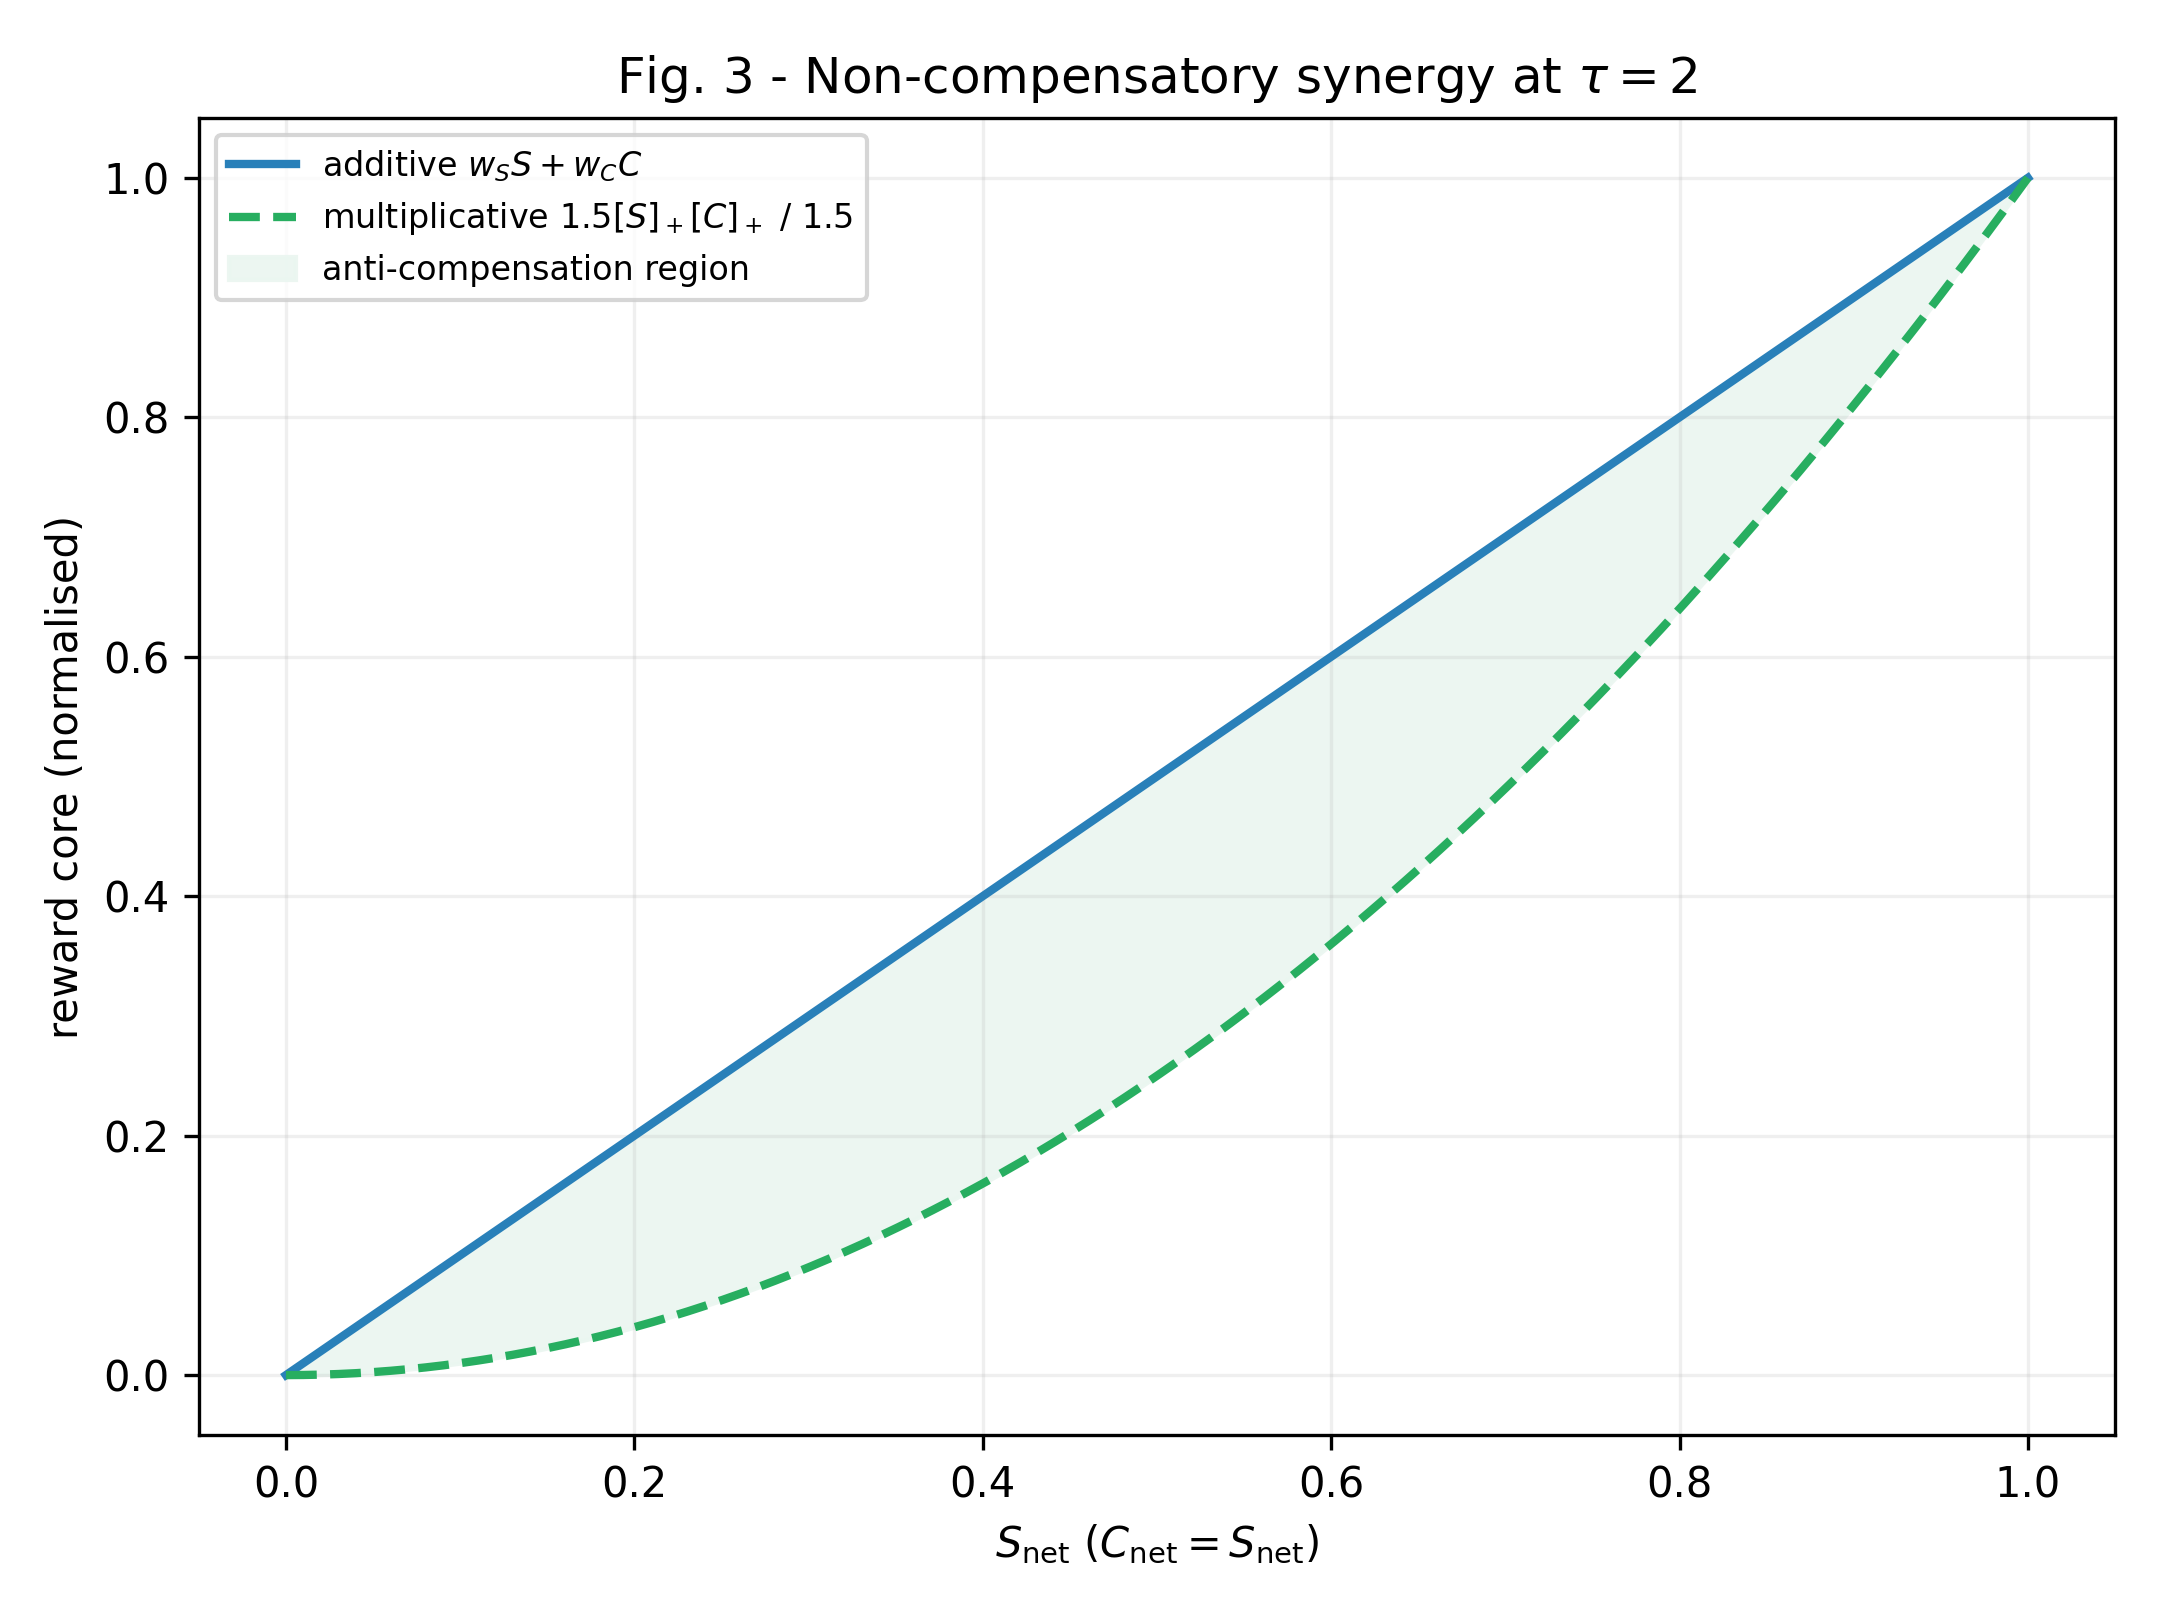
\includegraphics[width=0.78\linewidth]{figures/Figure_3_Synergy_Contour.png}
  \caption{Non-compensatory reward core at $\tau=2$. The multiplicative term $1.5[S_{\mathrm{net}}]_+[C_{\mathrm{net}}]_+$ (solid lower curve, scaled by $1/1.5$ for comparison) stays below the additive core and vanishes when either index collapses, whereas the additive core remains positive. Generated by \texttt{simulate\_benchmark.py} from Eq.~\eqref{eq:unified_objective}.}
  \label{fig:synergy}
\end{figure}

\begin{figure}[t]
  \centering
  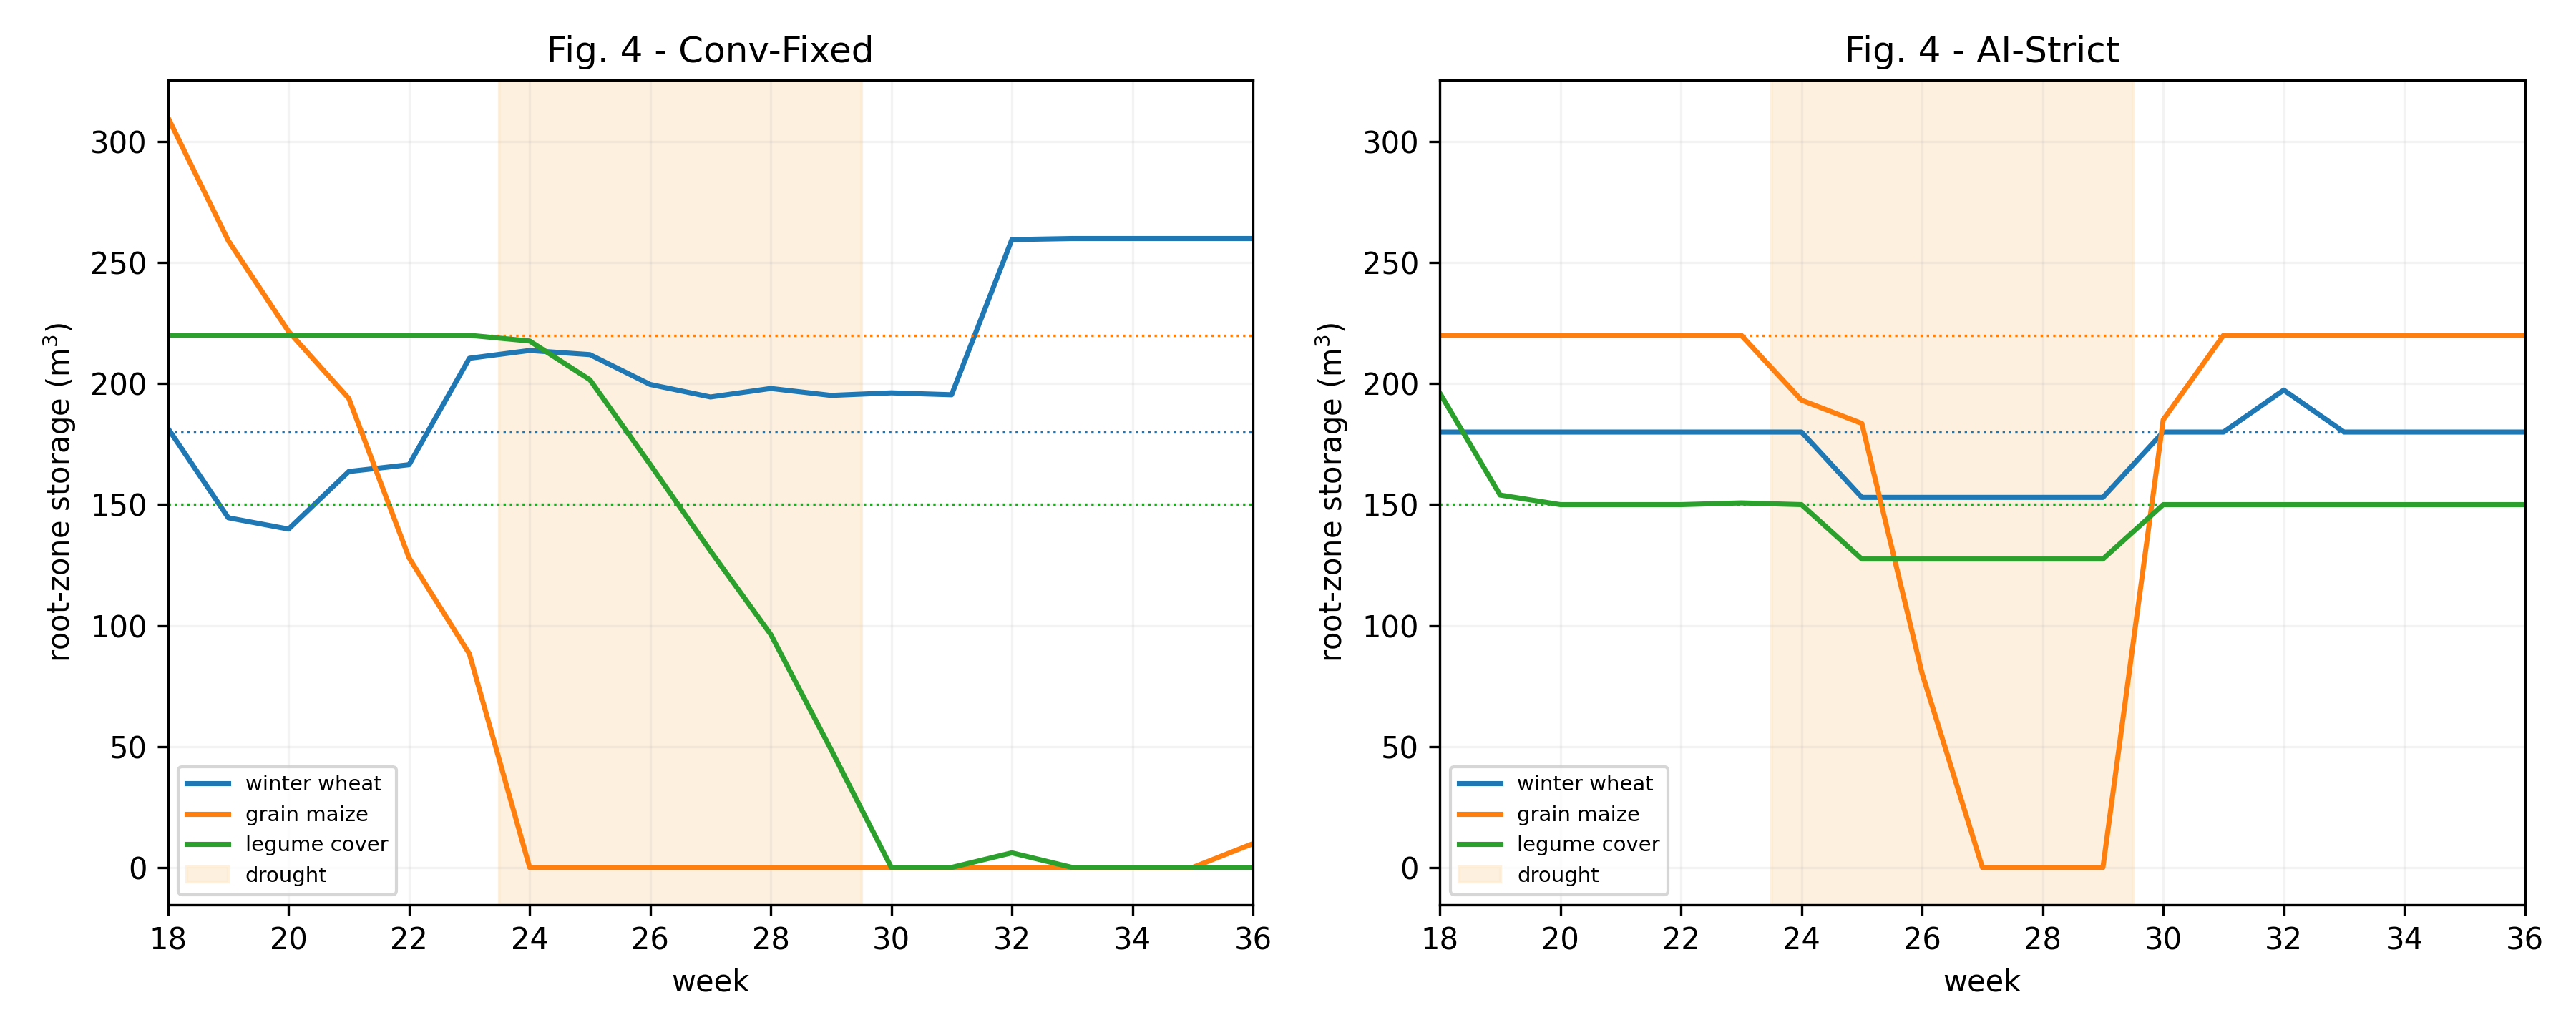
\includegraphics[width=\linewidth]{figures/Figure_4_Drought_Stress_Test.png}
  \caption{Drought trajectories for a representative seed (105). Root-zone storage is shown for the three crop groups with their critical floors (dotted); the shaded band is Weeks~24--29. \texttt{Conv-Fixed} cannot prevent severe depletion, while \texttt{AI-Strict} holds the two highest-priority plots near their survival caps. Generated by \texttt{simulate\_benchmark.py}.}
  \label{fig:drought}
\end{figure}

\begin{figure}[t]
  \centering
  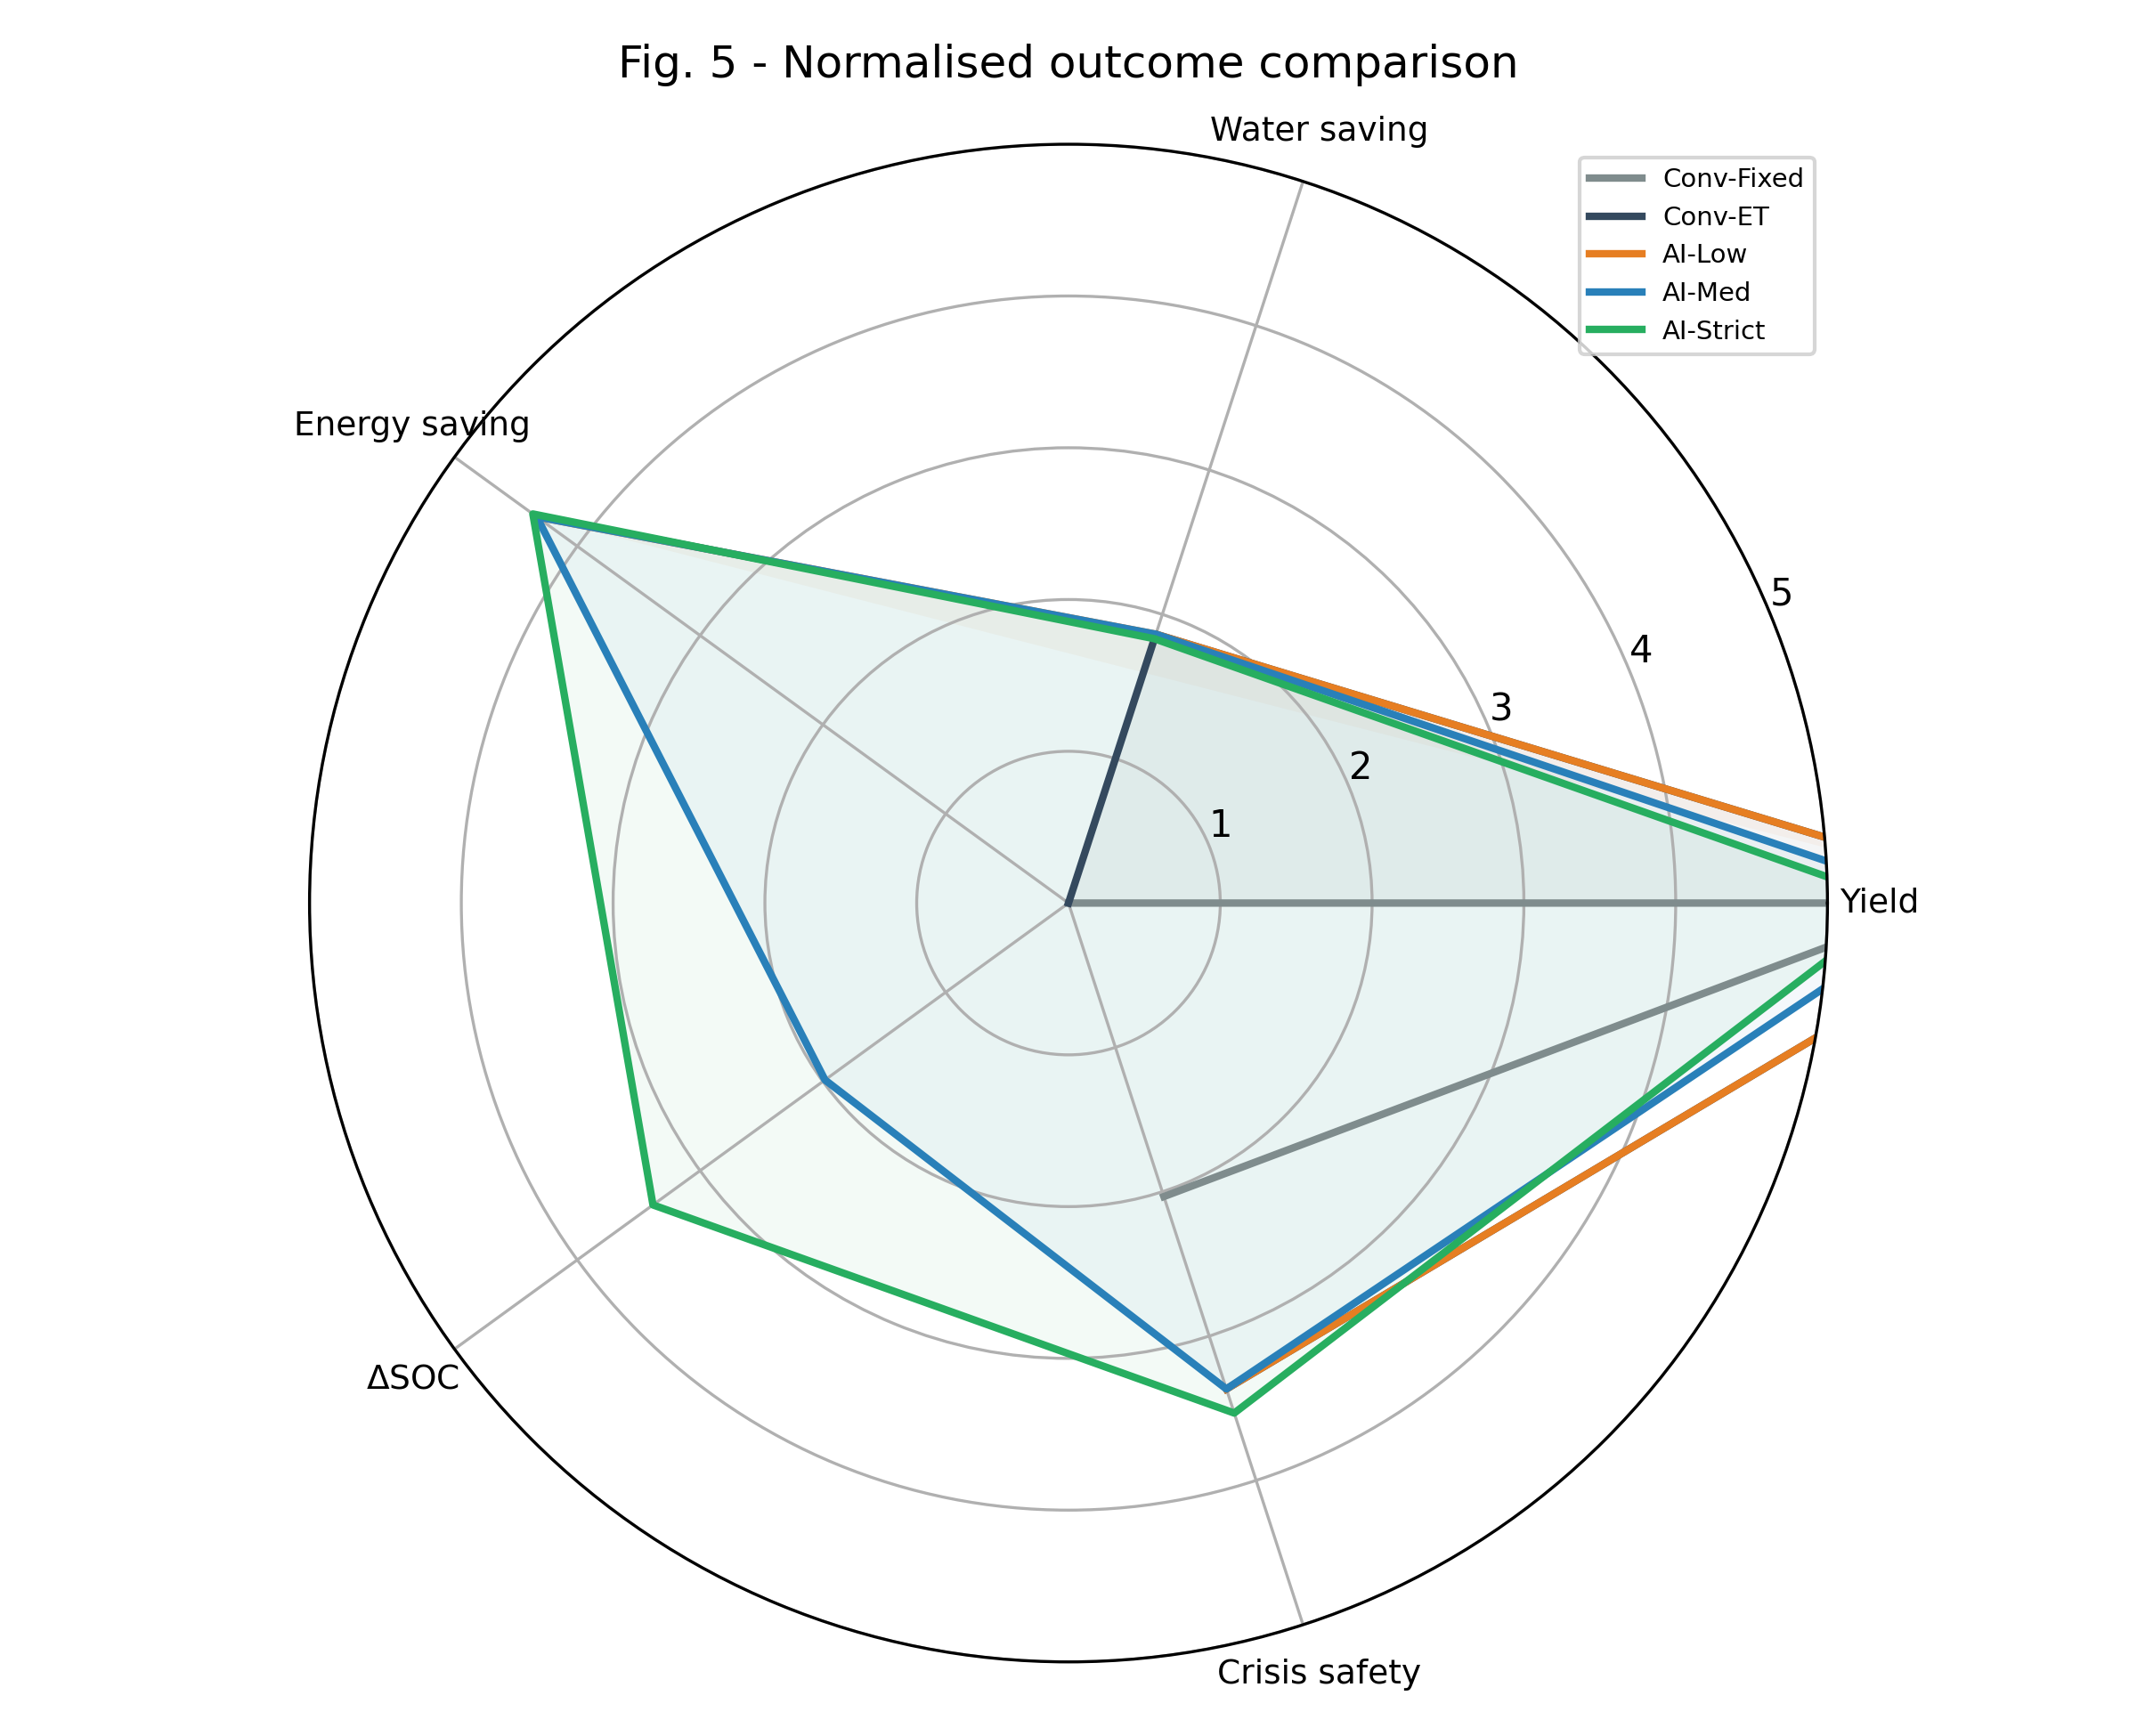
\includegraphics[width=0.78\linewidth]{figures/Figure_5_Radar_Comparison.png}
  \caption{Normalised five-pillar comparison (each axis scaled to $[0,5]$). Water and energy saving are relative to \texttt{Conv-Fixed}; crisis safety is $5$ minus crop-loss crop-weeks divided by three. The radar summarises Table~\ref{tab:results} and is generated by \texttt{simulate\_benchmark.py}.}
  \label{fig:radar}
\end{figure}

\begin{figure}[t]
  \centering
  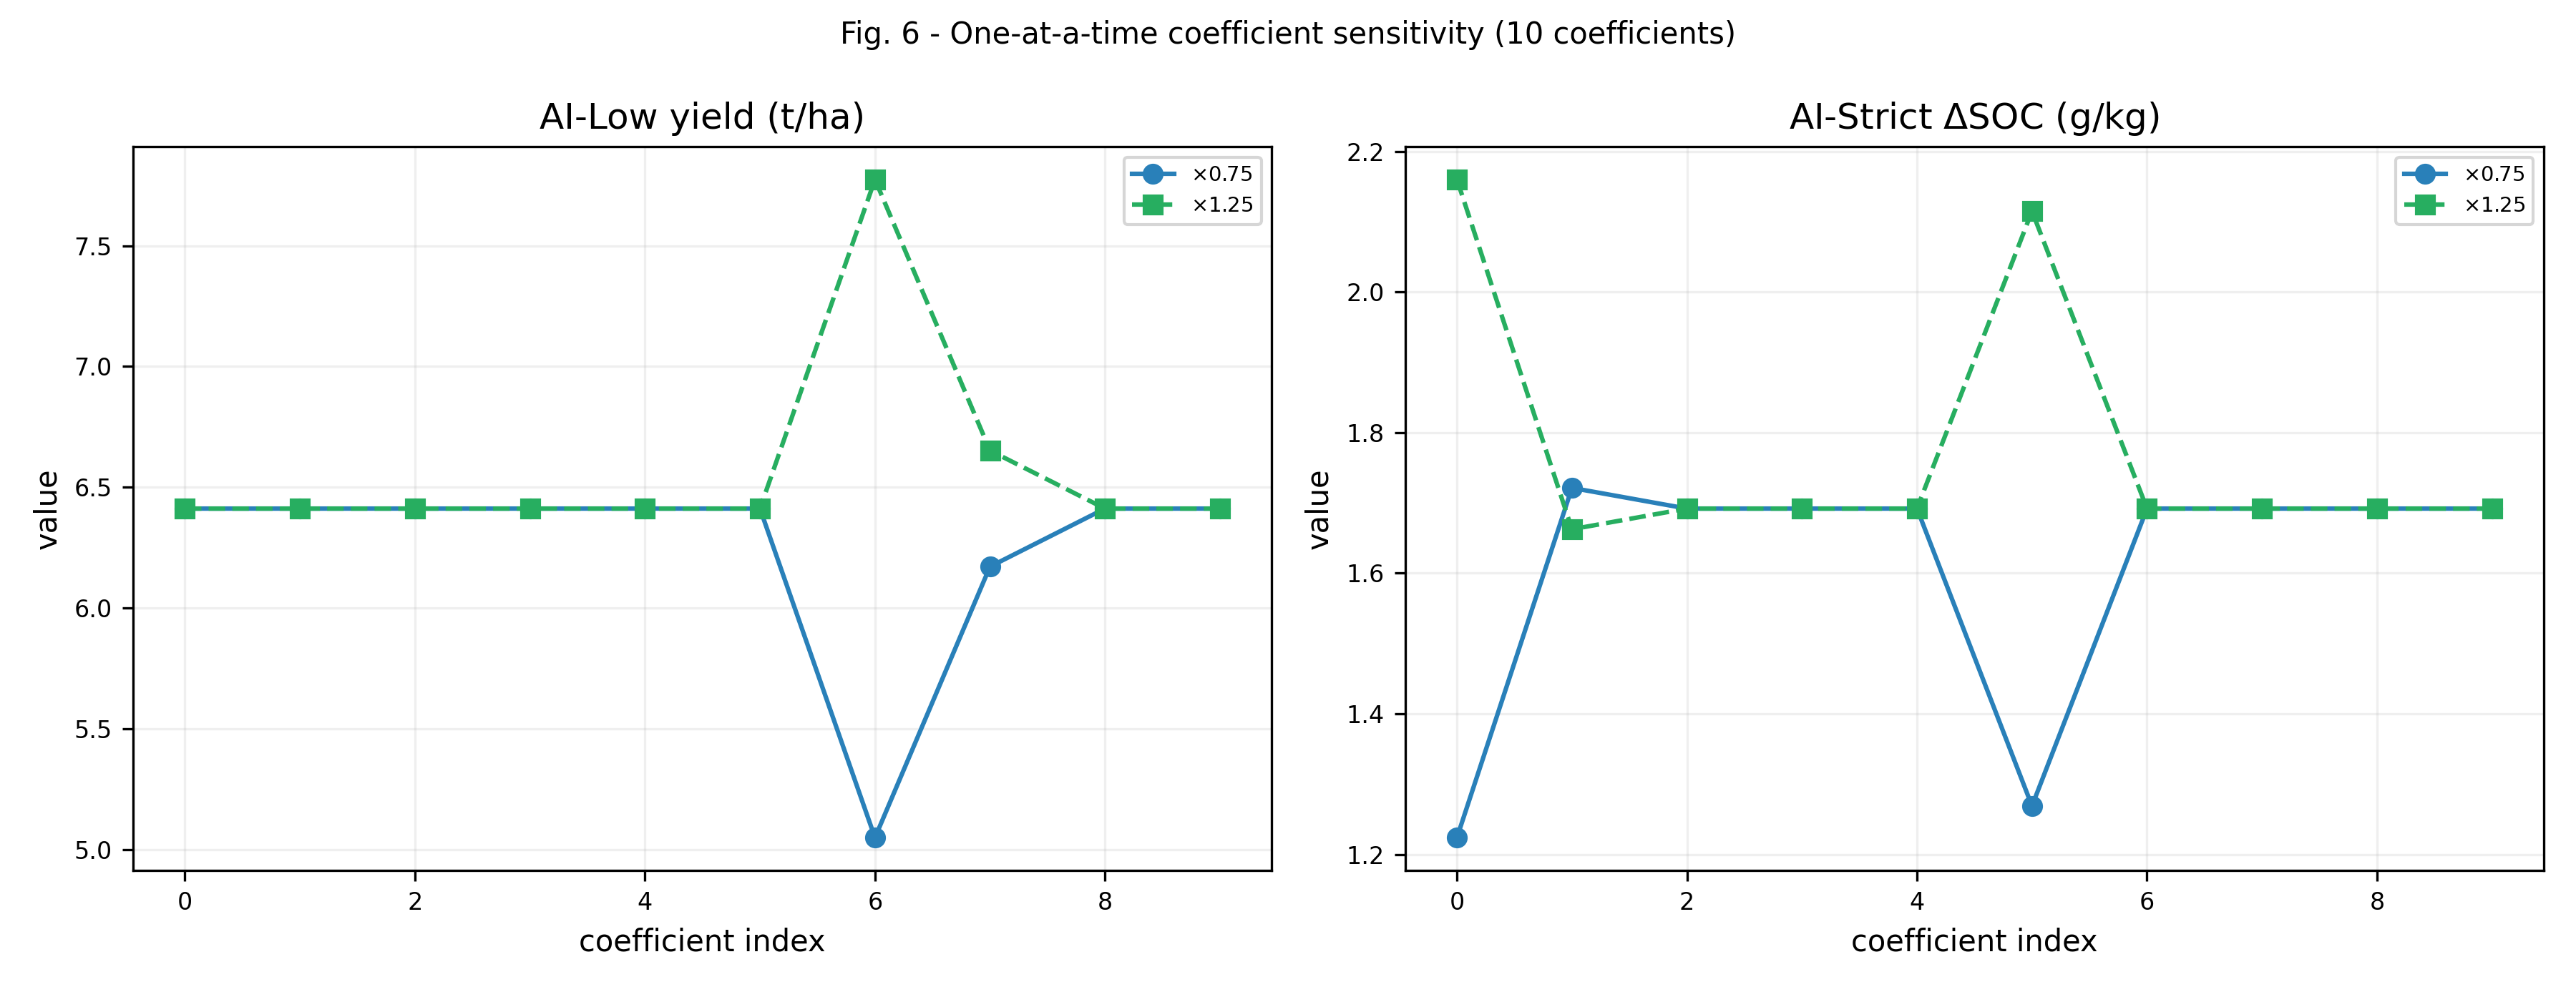
\includegraphics[width=\linewidth]{figures/Figure_6_Sensitivity.png}
  \caption{One-at-a-time sensitivity of three headline outcomes to $\pm25\%$ perturbations of the ten response coefficients (coefficient order as in Table~\ref{tab:sensitivity}). The qualitative conclusions C1--C4 do not change. Generated by \texttt{simulate\_benchmark.py}.}
  \label{fig:sensitivity}
\end{figure}

%----------------------------------------------------------------------
\section{Discussion and Limitations}
%----------------------------------------------------------------------
\subsection{Operational Tier Selection}
The three strictness tiers correspond to distinct agronomic transition stages. \texttt{AI-Low} ($\tau=0$) is a sensing-and-allocation tier: it changes duty cycling but leaves chemical intensity at the conventional $120$\,kg/ha, and its yield and irrigation are identical to \texttt{Conv-ET}. \texttt{AI-Med} ($\tau=1$) balances commercial productivity with a moderate chemical cap ($45$\,kg/ha) and captures about $60\%$ of the soil-carbon gain at a small yield cost. \texttt{AI-Strict} ($\tau=2$) is designed for water-stressed or ecologically sensitive zones where soil-capital preservation and drought triage supersede short-term output maximisation: it attains the highest $\Delta$SOC and fewest crop-loss events at the largest yield cost. Section~6 confirms this interpretation, and the paired statistics show that these differences are not seed-noise artefacts.

\subsection{Limitations and Future Empirical Validation}
Four limitations bound the scope of this work. First, the evaluation is a simulation benchmark rather than a multi-season field trial: the yield, soil-carbon and stress responses in Section~3.2 are parsimonious response functions, not calibrated crop models, and parameter transfer to other pedoclimates requires lysimeter and sensor-testbed validation. Second, although all ten coefficients survive $\pm25\%$ one-at-a-time perturbations (Section~6.1), this is not a global sensitivity analysis and does not establish parameter identifiability; the absolute g/kg and t/ha magnitudes remain illustrative. Third, edge execution of state estimation and triage logic introduces local microcontroller compute overhead that is not included in the reported radio-duty savings; hardware-in-the-loop profiling remains necessary. Fourth, the drought disturbance is a six-week level shift applied identically to all policies, so it tests triage mechanics but not sequence-dependent drought onset, recovery hysteresis or multi-year carry-over of soil carbon. Extending the protocol along those axes is the natural next step.

%----------------------------------------------------------------------
\section{Conclusion}
%----------------------------------------------------------------------
We presented a mathematically consistent, multi-tier agri-ecological optimization framework ($\tau \in \{0,1,2\}$) that resolves sign-inversion bugs in multiplicative sustainability cores via positive-part clipping, corrects unit-interval quadratic under-penalization via the monotone concave map $\psi_\tau(x)$, disambiguates hydrological storage ($\theta_{\mathrm{root},k,t}$) from depletion flux ($D_t^+$), and formalizes the nature gate $\Inatt^{(\tau)}$ alongside a deterministic drought triage fallback rule. A fully specified 52-week, 20-seed benchmark was executed against two conventional baselines: ET-scheduled irrigation cut water use by $37\%$ and raised yield by $11\%$ relative to fixed-rate scheduling, while adaptive duty cycling cut IoT energy by $87\%$ with no further water or yield cost. The strictness ladder then traded yield for soil carbon and drought safety, with \texttt{AI-Strict} delivering the highest $\Delta$SOC ($+1.69$\,g/kg) and the fewest crop-loss events ($4.40$ crop-weeks); paired tests and 20 coefficient perturbations support the orderings. By anchoring cross-policy comparison on physical agro-ecological metrics rather than incomparable dimensionless scores, the framework provides both a rigorous specification and reproducible baseline evidence for sustainable precision agriculture.

\section*{Statements and Declarations}
\noindent\textbf{Code and Data Availability:} All code and data required to reproduce the results and every figure are publicly available at \url{https://github.com/OsamaGharibElwaly/multi-tier-agri-ecological-optimization-framework} under the MIT licence. The repository contains \texttt{scripts/simulate\_benchmark.py} (five-policy benchmark, Tables~\ref{tab:results}, \ref{tab:paired}, \ref{tab:diagnostics}, \ref{tab:sensitivity} and Figs.~\ref{fig:synergy}--\ref{fig:sensitivity}), \texttt{scripts/generate\_figures.py} (Figs.~\ref{fig:architecture}--\ref{fig:tiers}), \texttt{results/results.json} (all 100 per-seed records: 5 policies $\times$ 20 seeds), the four generated \texttt{results/*\_table.tex} files, and \texttt{README.md}. The scripts require NumPy, SciPy and Matplotlib; from the repository root run \texttt{python scripts/simulate\_benchmark.py} and \texttt{python scripts/generate\_figures.py}. A version-archive DOI will be assigned at acceptance.\\
\noindent\textbf{Funding:} The author declares that no specific external funding was received for this work.\\
\noindent\textbf{Competing Interests:} The author declares no competing interests.

\begin{thebibliography}{9}

\bibitem{karakatsanis_2026}
G.~Karakatsanis, D.~Managoudis, and E.~Makronikolakis, ``REGENA: Growth Function for Regenerative Farming,'' \emph{Agriculture}, vol.~16, no.~1, art.~134, 2026. DOI: \texttt{10.3390/agriculture16010134}.

\bibitem{buckton_2023}
S.~J. Buckton, I.~Fazey, B.~Sharpe, \emph{et~al.}, ``The Regenerative Lens: A conceptual framework for regenerative social--ecological systems,'' \emph{One Earth}, vol.~6, no.~7, pp.~824--842, 2023. DOI: \texttt{10.1016/j.oneear.2023.06.006}.

\bibitem{gerndt_2025}
M.~Gerndt, M.~Ispir, I.~D.~N{\'u}{\~n}ez Araya, and S.~Benedict, ``Energy-Aware Duty Cycle Management for Solar-Powered IoT Devices,'' \emph{Sensors}, vol.~25, no.~14, art.~4500, 2025. DOI: \texttt{10.3390/s25144500}.

\bibitem{dhall_2018}
R.~Dhall and H.~Agrawal, ``An Improved Energy Efficient Duty Cycling Algorithm for IoT based Precision Agriculture,'' \emph{Procedia Computer Science}, vol.~141, pp.~135--142, 2018. DOI: \texttt{10.1016/j.procs.2018.10.159}.

\bibitem{water_2026}
Z.~Fu, C.~Zhang, X.~Liu, J.~Tian, and Y.~Song, ``Mitigating Peak Edge Effects in Multi-Zone Irrigation: A Safety-Constrained Reinforcement Learning Approach with Short-Term Evapotranspiration Forecasting,'' \emph{Water}, vol.~18, no.~8, art.~988, 2026. DOI: \texttt{10.3390/w18080988}.

\bibitem{agrieng_2025}
Z.~Wang, S.~Xiao, J.~Wang, A.~Parab, and S.~Patel, ``Reinforcement Learning-Based Agricultural Fertilization and Irrigation Considering N\textsubscript{2}O Emissions and Uncertain Climate Variability,'' \emph{AgriEngineering}, vol.~7, no.~8, art.~252, 2025. DOI: \texttt{10.3390/agriengineering7080252}.

\bibitem{frontiers_water_2025}
L.~K{\aa}ge, V.~Mili{\'c}, M.~Andersson, and M.~Wall{\'e}n, ``Reinforcement learning applications in water resource management: a systematic literature review,'' \emph{Frontiers in Water}, vol.~7, art.~1537868, 2025. DOI: \texttt{10.3389/frwa.2025.1537868}.

\bibitem{sos_food_2025}
S.~te Wierik, F.~DeClerck, A.~H.~W.~Beusen, D.~Gerten, F.~Maggi, A.~Norberg, K.~J.~Noone, L.~Schulte-Uebbing, M.~Springmann, F.~H.~M.~Tang, W.~de Vries, D.~P.~van Vuuren, S.~J.~Vermeulen, and J.~Rockstr\"om, ``Identifying the safe operating space for food systems,'' \emph{Nature Food}, vol.~6, no.~12, pp.~1153--1163, 2025. DOI: \texttt{10.1038/s43016-025-01252-6}.

\bibitem{ca_boundaries_2026}
J.~Rockstr\"om, A.~Kassam, T.~Friedrich, D.~C.~Reicosky, J.~Dumanski, T.~W.~Goddard, and R.~A.~Peiretti, ``Conservation agriculture: helping to return to within planetary boundaries,'' \emph{Global Sustainability}, vol.~9, 2026. DOI: \texttt{10.1017/sus.2025.10045}.

\bibitem{jalrakshak_2026}
P.~Chowdhury, ``TRUST THE SOIL, NOT ONLY THE SENSOR: WATER-BALANCE INTEGRITY CHECKING AND RISK-TRIGGERED SENSING FOR RESILIENT, LOW-ENERGY IOT IRRIGATION,'' \emph{Acta Innovations}, vol.~63, no.~3s, 2026. DOI: \texttt{10.62441/actainnovations.vi.2634}.

\bibitem{iot_wakeup_2026}
D.~E.~Ruiz-Guirola, S.~Montejo-S\'anchez, I.~Leyva-Mayorga, Z.~Han, P.~Popovski, and O.~L.~Alcaraz L{\'o}pez, ``Energy Management and Wakeup for IoT Networks Powered by Energy Harvesting,'' \emph{IEEE Internet of Things Journal}, vol.~13, no.~9, pp.~18574--18591, 2026. DOI: \texttt{10.1109/jiot.2026.3664201}.

\bibitem{solar_iot_2026}
S.~Falamba, P.~G.~Home, S.~Ondimu, and E.~Bwambale, ``Development and validation of a solar-powered IoT drip irrigation system integrating multi-sensor monitoring and threshold control,'' \emph{Smart Agricultural Technology}, vol.~14, art.~102402, 2026. DOI: \texttt{10.1016/j.atech.2026.102402}.

\end{thebibliography}

\end{document}